%------------------------------------------------------------------------------
% Tesis de Maestria en Electrica.
%------------------------------------------------------------------------------

\documentclass[twoadviser,master]{labicetesis}

%%%%%%%%%%%%%%%%    Definicin de directorios de trabajo   %%%%%%%%%%%%%%%%%%%%


\newcommand{\DirFigP}{./Figures/Portada}
\newcommand{\DirFigA}{./Figures/Agradec}
\newcommand{\DirFigCuno}{./Figures/Capitulo1}
\newcommand{\DirFigCdos}{./Figures/Capitulo2}
\newcommand{\DirFigCtres}{./Figures/Capitulo3}
\newcommand{\DirFigCcuatro}{./Figures/Capitulo4}
\newcommand{\DirFigCcinco}{./Figures/Capitulo5}
\newcommand{\DirFigAa}{./Figures/ApendiceA}
\newcommand{\Ima}{./Pictures}
\newcommand{\figRef}[1]{\textbf{Figure} \ref{#1}}
\renewcommand{\citepunct}{; }

%%%%%%%%%%%%%%%%%%%%%%%%%    Datos personales    %%%%%%%%%%%%%%%%%%%%%%%%%%%%%%

\title{Diferential and double differential cross section of one pion production for CC neutrino interactions in the MINERvA's Tracker}		% Titulo del documento.
\author{Everardo Granados V\'azquez}				% Autor del documento.
\date{December, 2023}									% Fecha de publicacin.
\crest{\DirFigP/EscudoAltaCalidadjpgUG.eps}				% Escudo de la Universidad
\grade{DOCTORADO EN F\'ISICA }			% Grado o Titulo
\adviser{Dr. Juli\'an F\'elix}{Dra. Laura Fields}	%Asesor(es)
\bars{\DirFigP/porta3}									%Barras

\hyphenation{}
\clubpenalty=10000
\widowpenalty=10000

%==============================================================================
%==============================================================================
\begin{document}                        % Empieza el documento
% \bibliography{url}
 \pagenumbering{roman}
	\maketitle			% Portada
	\formatLabice			% Diseño de la hoja y Formato de tesis
	\chapter*{Agradecimientos Institucionales}
\label{Cap:Agr2}

\begin{itemize} 

\item A la \textbf{Universidad de Guanajuato}, por el apoyo que me brindó por medio de la rectoría del Campus Le\'on y la dirección de la División de Ciencias e Ingenierías para poder realizar mi estancia de investigación en Fermi National Accelerator Laboratory in Batavia, Illinois, Estados Unidos de Am\'erica.

\begin{figure}[h]
	\centering
	
\includegraphics[width=2.6cm,height=2.7cm]{\DirFigA/ug.eps}
\end{figure}

\item Al \textbf{Consejo Nacional de Ciencia y Tecnología (CONACyT)}, por el apoyo que me brindó al otorgarme la beca para posgrado. 

\begin{figure}[h]
	\centering	
	
\includegraphics[scale=0.26]{\DirFigA/conacyt.eps}
\end{figure}

\item To \textbf{Fermi National Accelerator Laboratory}, for all the support during my stay. To \textbf{MINERvA collaboration}, for all the guidance during my stay in Fermilab and all the support during my PhD.

\begin{figure}[h]
	\centering	
	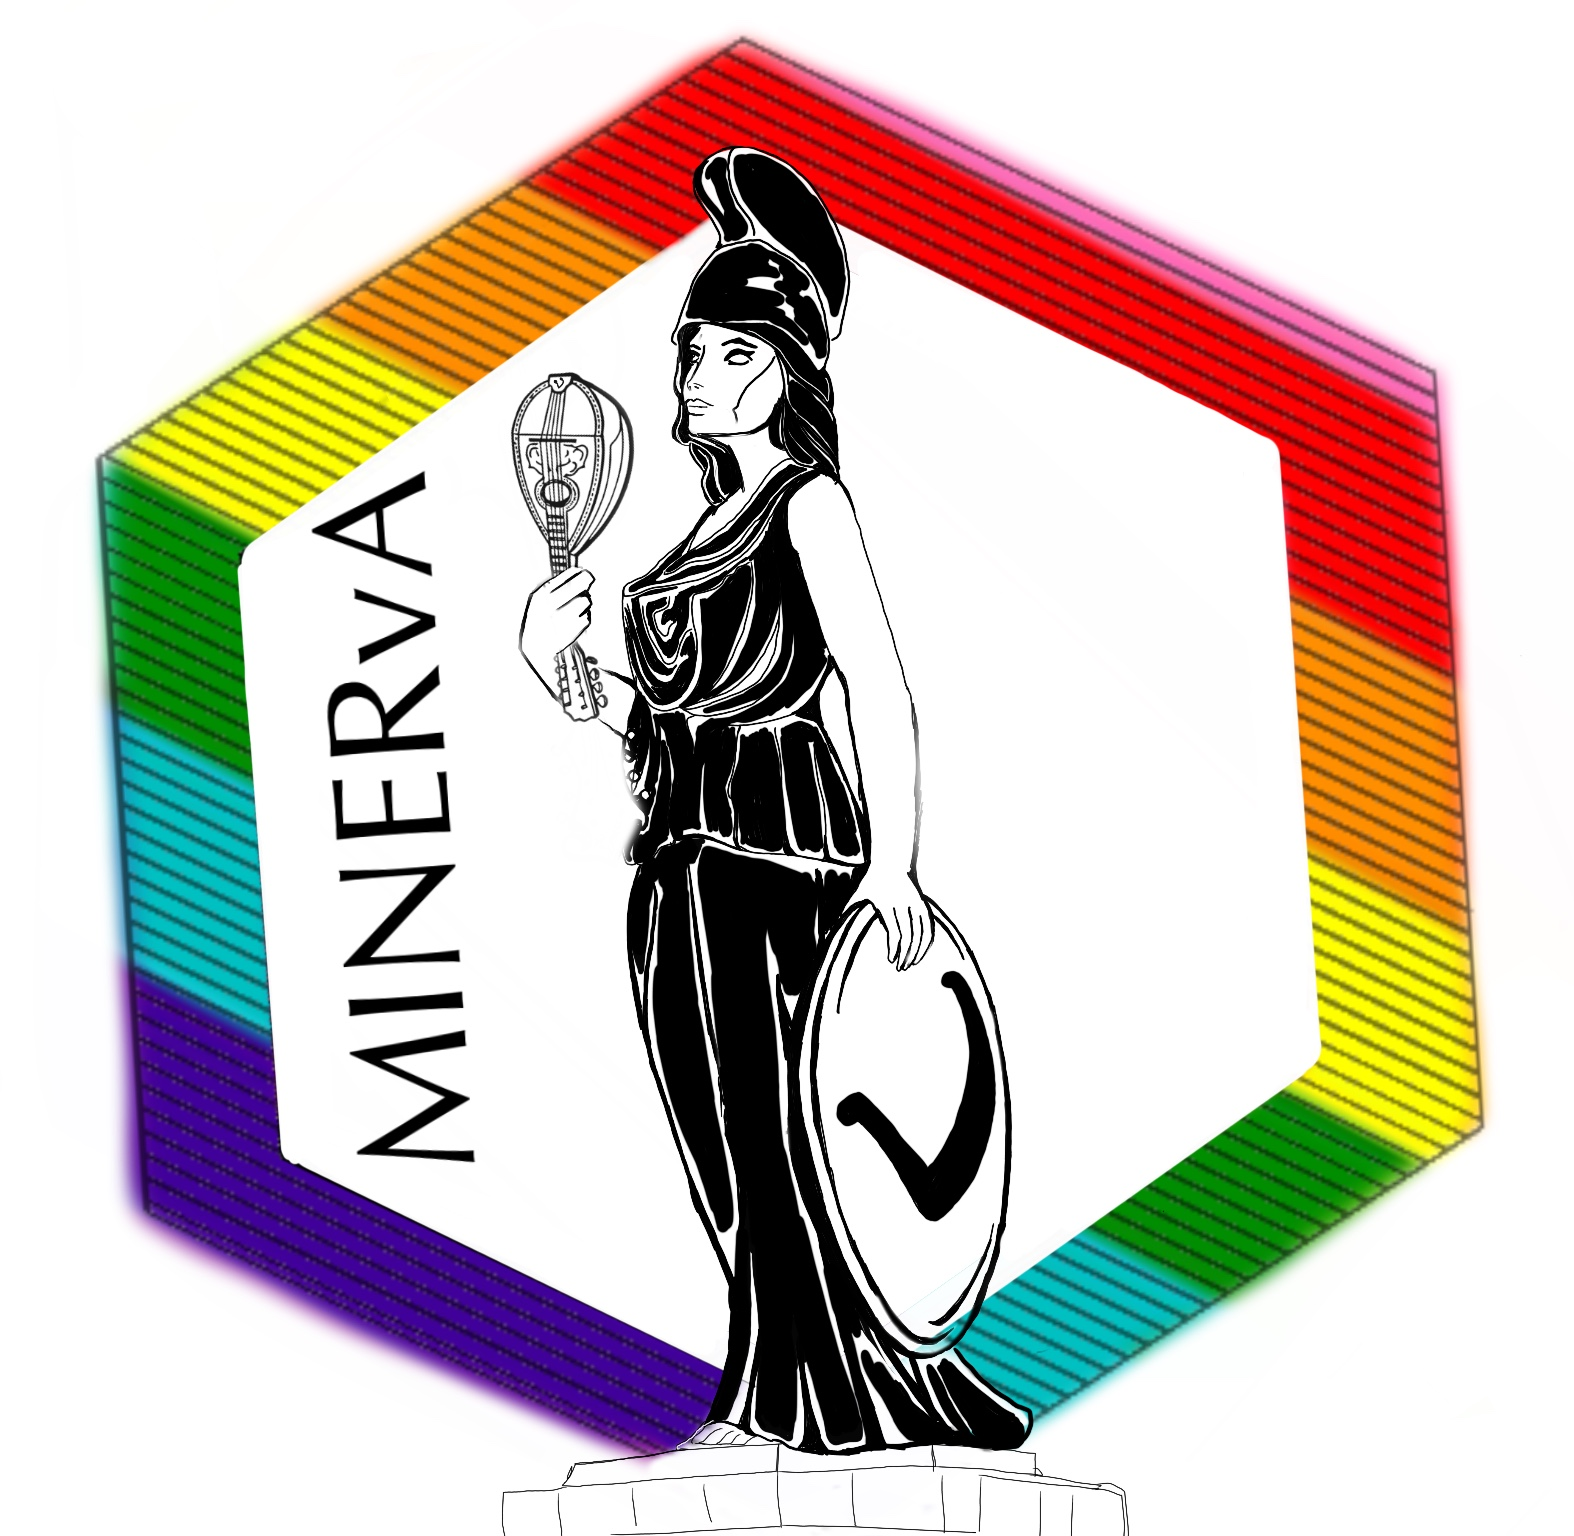
\includegraphics[scale=0.05]{\DirFigA/minerva_pride.jpeg}
    
\includegraphics[scale=0.30]{\DirFigA/FNAL_Logo.jpg}
\end{figure}

\end{itemize}

\newpage   % Agradecimientos Institucionales.
	\chapter*{Agradecimientos}
\label{Cap:Agr1}


	 
\newpage   % Agradecimientos.
	\section*{Abstract}
\label{Cap:Prlg1}
\it
Future and current neutrino oscillation experiments such as NO$\nu$A\cite{NOvA}, DUNE\cite{DUNE} and HyperK\cite{HyperK} require a precise measurement of neutrino interactions. These operate in the region of energy of a few GeV, where multiple interactions produce pions in the final state. Therefore, it is crucial to have a complete understanding of the pion production by charged current neutrino interactions.


Neutrino cross sections are one of the necessary ingredients to measure the rate of neutrino oscillation. Having this in mind, at the beginning of 2000's, the MINER$\nu$A experiment was designed with the aim to reduce cross section uncertainties and improve the nuclear models. This experiment has the capability to measure the cross section from diverse types of interactions on 6 different materials. The detector was located on the axis of the NuMI beam where the mean neutrino energy for the Low Energy era was 3 GeV and for the Medium Energy era 6 GeV. 

The results presented in this thesis show the measurement of single differential (1D analysis) and double differential (2D analysis) cross sections for charged current muon-neutrino interactions that produce one pion in the final state in the MINER$\nu$A tracker (hydrocarbon) with a neutrino beam of $<E_\nu> = 6$ GeV. 

The 1D analysis shows results for regions of pion kinetic energy never shown before in previous analyses. It implements a new pion reconstruction algorithm that allows the measurement of the kinetic energy and pion angle for pions without a track in the detector. Combining the old and the new technique, the data selection efficiency increases from 6\% to 11\% with a minimal effect to the purity.

The 2D analysis shows the first double differential cross section for pion production in MINER$\nu$A. This analysis shows the combination of lepton variables with hadronic variables. The results of this analysis are compared with the tuned version of GENIE v2.12.6. The production of these results brings a better understanding of the cross section for specific kinematic regions.  



\normalfont

\newpage			  % Prologo

	\dominitoc
	\tableofcontents                      % Índice general
	\listoffigures                        % Índice de figuras
	\listoftables                         % Índice de tablas
	\newpage


%&&&&&&&&&&&&&&&&&&&&&&&&&&&&&&&&&&&&&&&&&&&&&&&&&&&&&&&&&&&&&& &&&&&&&&&&&&&&&
%       Capitulos
%&&&&&&&&&&&&&&&&&&&&&&&&&&&&&&&&&&&&&&&&&&&&&&&&&&&&&&&&&&&&&&&&&&&&&&&&&&&&&&
	\pagenumbering{arabic}
	\parskip = 0.5cm			%espacio entre parrafos
	\chapter{Introduction}
\minitoc
\label{Cap:Int}
%%%%%%%%%%%%%%%%%%%%%%%%%%%%%%%%%%%%%%%%%%%%%%%%%%
% 
\section{Standard Model}
\label{Cap:Int:SM}
The Standard Model of Particles (SM) is a unified quantum field theory of the electroweak interaction and Quantum Chromodynamics (QCD). It models fundamental objects, quantum fields, that represents 17 fundamental particles, with their respective antiparticles.

The elementary particles are divides in two meanly blocks: 
\begin{itemize}
    \item The fermions, these particles are commonly know as the matter particles (or antimatter particles). These are fractional spin particles and are divides in two mainly blocks, quarks and leptons. These are described in more depth later. 
    \item The bosons, these particles are the carriers of the weak, strong and electromagnetic fundamental interactions. The Higgs field, it is a field that supplement the SM by the Higgs mechanism to generate masses to the bosons and fermions. These are described in more depth later.
\end{itemize}

The agreement of the SM predictions with most precise measurements of the particle experiments, provides a high confidence in this model. However, it is not complete, there are phenomena that are not described by it, such as the case of dark mater and neutrino oscillations.

\begin{figure}[!htb]
\centering
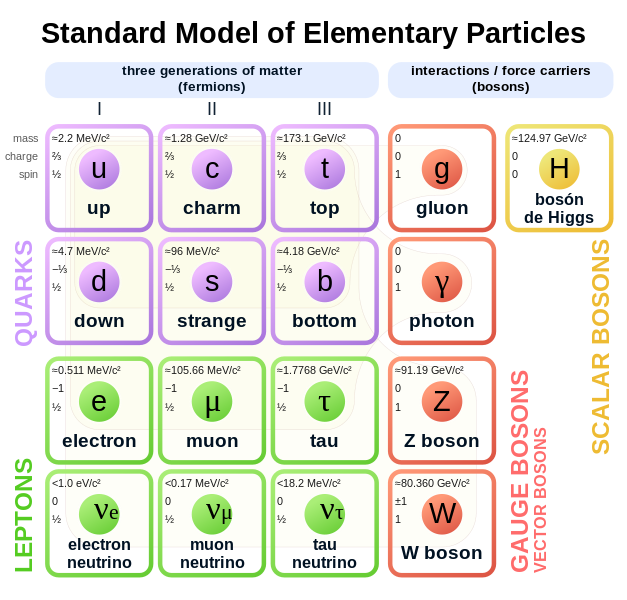
\includegraphics[scale=0.5]{Figures/Chapter1/Standard_Model_of_Elementary_Particles.png}

        \caption{In the figure is shown a pictorial summary of the standard model. In this are shown the the 17 particles of the SM. Something that should be considered is that there are other 17 that correspond to the antiparticle of each particle. Figure from \cite{SM_Table}} 
\label{fig:SM}
\end{figure}
 
\subsection{Bosons}
Bosons and fermions are differentiated by their spin characteristics. Bosons have integer values for spin, while fermions have half-integer values. In the SM, the elementary particles interacts through the gauge bosons, which acts as carriers for the fundamental forces of weak, strong and electromagnetic interactions. The Higgs boson plays a crucial role in the Higgs Mechanism, whereby particles gain mass through their interaction with this boson. Additionally, there is a hypothetical boson called as graviton, this particle should be the carrier of the gravitational force, it have no been observed yet \textbf{Agregar bibliografia}.  

\subsubsection{The electromagnetic force}
Described by the quantum electrodynamics, the electromagnetic force is transmitted by photons, which interact exclusively with charged spin 1/2 particles. The mass of the photons is 0. This force is capable of acting over long distances. These are the responsible of  The effects of electromagnetic force are observable on a macroscopic scale, and it finds numerous practical applications.

\subsubsection{Strong Force}
It is carried by the gluons, these are the responsible to joint quarks and generate hadrons. This force is also the responsible to joint the neutrons and protons in the interior of the atomic nucleus. The interactions mediated by strong force are modeled by the Quantum Chromodynamics (QCD). Here the charge is represented as "color", which is carried only by quarks.

In QCD, There are three color charges (red, blue and green). The quarks has one charge color and the gluons are has two colors. In the strong interactions the color of thee quarks may change but as the same with the electric charge the color is always conserved. Unlike photons, the gluons are capable to interact with other gluons this make more complicated the consider all the interactions that    
 

\subsubsection{The weak force}
It is carried by the bosons $W^\pm$ and $Z$. This force is the responsible of various particles decays and in some scattering processes. All the elementary fermions may interacts by this force, in the case of the neutrinos it is the only known way that this particle interacts.

There are two types of interactions, the Charge Current (CC) interaction an the Neutral Current (NC) interaction. The CC interactions occurs when particles interacts by the $W^\pm$ boson, In this tipe of interaction 

\subsection{Fermions}
These are the blocks of the matter, 12 of the 17 fundamental particles are Fermions, these are defined as particles with half integer spin. These are divided in quarks and  leptons. 

\textbf{Quarks}
The quarks are described by the QCD, it is a gauge theory based on SU(3) symmetry.  

\textbf{Leptons}
In the SM are 6 different leptons known, with their respective antiparticles. These are divided in 3 groups called generations, these can be represented doublets: 

$\begin{pmatrix}
    \nu_e \\
    e^-
\end{pmatrix}$, 
$\begin{pmatrix}
    \nu_\mu \\
    \mu^-
\end{pmatrix}$, 
$\begin{pmatrix}
    \nu_\tau \\
    \tau^-
\end{pmatrix}$

The electron $e^-$, muon $\mu^-$ and tau $\tau^-$ are electrical charged leptons; with a charge $-e$, were $e$ is the magnitude of charge of the electron , these leptons interact by electromagnetic and weak forces. 

The $\nu_e$, $\nu_\mu$ and $\nu_\tau$ are electrical neutral leptons, this only interacts by weak force. These leptons are known as neutrinos and depend the generation these are called electron-neutrino ($\nu_e$), muon-neutrino ($\nu_\mu$) or tau-neutrino. 

\subsection{Neutrinos}
The neutrinos are the most abundant particles with mass in the universe of the SM. These are leptons, with out electrical charge. 

\subsubsection{Brief story of the neutrinos}
During the beginning of last century, the nuclear physicist studied the radioactivity of different materials. During this studies the identify meanly 3 types of nuclear decays: $\alpha$-decay, $\beta$-decay and the $\gamma$-decay. The energy of the  $\alpha$-decay and $\gamma$-decay is discrete and depend of the atomic nucleus that emits the radiation. The spectrum energy shows characteristic picks for certainly values of energy, in the \textbf{Figure} \ref{fig:abgSpectrum} two examples of energy spectrum for alpha and gamma emissions are shown. On the other hand, the $\beta$-decay processes produce a continuum spectra, in the \textbf{Figure} \ref{fig:abgSpectrum}an example of $\beta$-decay energy spectrum is shown. The fact that the energy spectrum of the $\beta$-decay electron is a continuum represents that a portion of the energy were lost or a violation of the energy conservation law.

\begin{figure}[!htb]
\centering
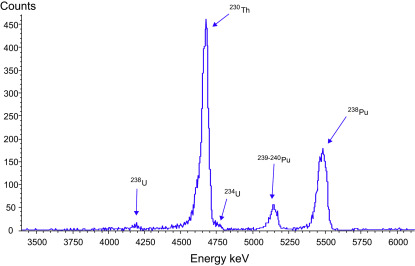
\includegraphics[scale=0.8]{Figures/Chapter1/alphaspectrum.jpg}
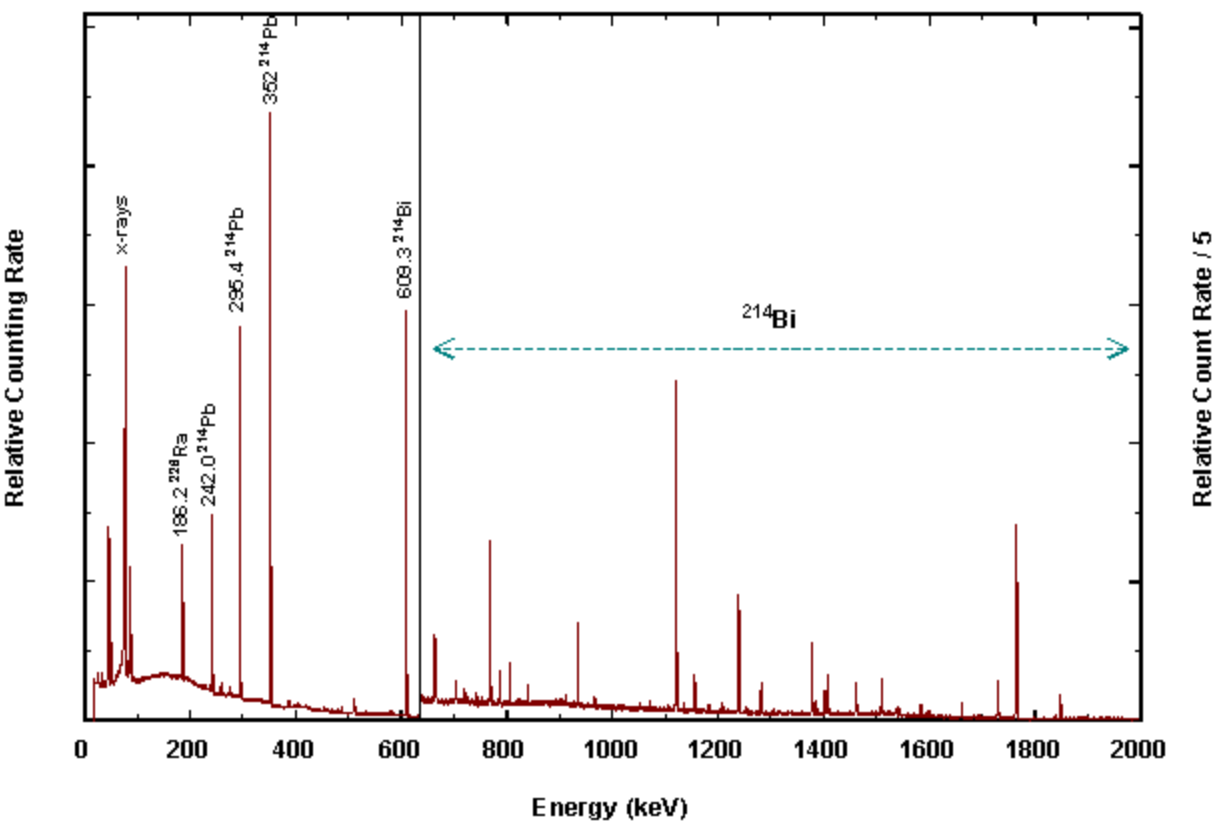
\includegraphics[scale=0.2]{Figures/Chapter1/radspec_gamma.png}
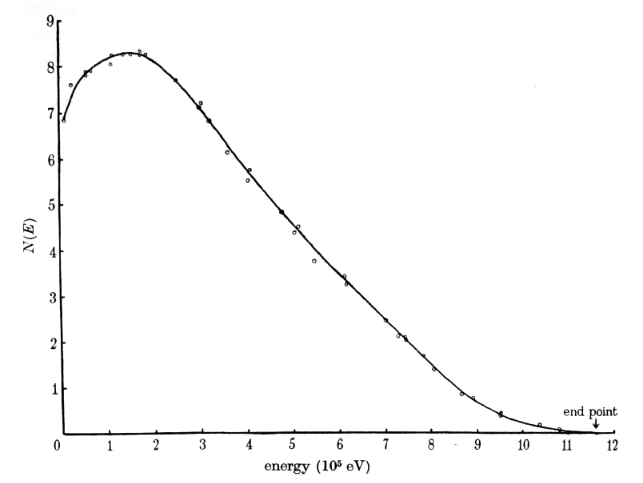
\includegraphics[scale=0.25]{Figures/Chapter1/Ra_betaSpec.png}

        \caption{Top plot, alpha spectrum of mixture of radioactive materials measured by a gas detector\cite{alphaSpectrum}. Middle plot, gamma spectrum of Radium-226 from high purity germanium detector\cite{RaSpectrum_gamma}. Bottom plot, spectrum of energy of electron from beta decay in of Ra\cite{Ra_betaSpec}} 
\label{fig:abgSpectrum}
\end{figure}

In 1930 Wolfgang Pauli \cite{NeutrinoHistory} proposed in a letter that the continuum spectra might be due to one more "invisible" light neutral particle, this should have spin 1/2 and obey the exclusion principle, he call this particle \textit{neutrons}. In the letter Pauli explain that with this particle the electron would be able to take any momentum until the maximum limit allowed ant the other particle has the residual momentum. In 1932 Chadwick discovered the neutron, it did not match with the Pauli description. In 1933, Enrico Fermi adopted the name of \textit{neutrino} for the particle proposed by Pauli; Fermi propoused a model where the neutrino should be a $^1/_2$ spin particle (a fermion). In 1953 the neutrinos were observed by the experiment of Clyde Cowan and Frederick Reines \textcolor{red}{Agregar referencia del descubrimiento del neutrino}. In this experiment they measured the anti-neutrinos produced in Savanna River Reactor in South Carolina and they show that .

\section{Neutrino interactions}
\label{Cap:Int:NuInteractions}

\section{Neutrino Oscillation}
\label{Cap:Int:NuOscillation}

\section{CC $\nu$ single pion production status}
\label{Cap:Int:Motivation}


 


	%%%%%%%%%%%%%%%%%%%%%%%%%%%%%%%%%%%%%%%%  NuMI  %%%%%%%%%%%%%%%%%%%%%%%%%%%%%%%%%%%%%%%%%%%%%%%%%%%
\chapter{MINER$\nu$A Experiment}
\minitoc
\label{Cap:MnvExperiment}

\section{Introduction}
\label{Chap2:MnvExperiment:Intro}
MINER$\nu$A is a neutrino experiment that has as main goal measure the neutrino cross section on 6 different materials, such as lead (Pb), iron (Fe), water ($H_2O$), carbon (C), plastic scintillator and (CH) and Helium (He). This with the aim to use the obtained results to improve nuclear models which would be used in future neutrino oscillation experiments. The MINER$\nu$A detector was located in the MINOS Near Detector building (MINOS Hall) in the neutrino campus in Fermilab 100 m underground with the aim to remove the cosmic rays background in the line of the neutrino beam produced by NuMI. It was located upstream to the MINOS ND, MINER$\nu$A was not an magnetized detector, in this way MINER$\nu$A could use to MINOS ND as muon spectrometer, reducing the uncertainties of muon charge and momentum.  

The experiment starts to take data from 2009 to 2019. For the first 3 years (2009-2012) taking data with the mode Low Energy (LE) neutrino beam ($<E_\nu>=3$ GeV) and in the Medium Energy (LE) mode ($<E_\nu> = 6$ GeV) during the following years (2013-2019). The total number of Protons on Target (POT) that produced the neutrino beam were $16.1\times10^{20}$ in neutrino mode and $14.1\times10^{20}$ in the antineutrino mode. 

\section{NuMI Beam}
\label{Cap:MnvExperiment:NuMI}
The Neutrino at the Main Injector \cite{Numi} (NuMI) neutrino beam is a facility that has provided neutrinos to experiments such as MINOS\cite{MINOS}, COSMOS\cite{COSMOS}, MINER$\nu$A\cite{MINERvA}, ArgoNeut\cite{ArgoNeuT}, NOvA\cite{NOvA}, MINOS+\cite{MINOS+} and more recently ArgonCube 2x2\cite{twobytwo}.

The NuMI beam facility provides neutrino and antineutrinos to the different experiments colliding a proton beam of 120 GeV against a graphite target. The charged hadron produced are  focused by two to magnetic horns. Depending the direction of the electrical current in the horns neutrinos or antineutrinos are produced in the resulted beam. The horn focused the hadrons throughout the decay pipe and during the travel most part of these hadrons decays in a neutrino and other charged particles. Most part of the remnant charged particles are absorbed by the rock, obtaining in this way an intense neutrino beam passing through the rocks.  

\begin{figure}[!htb]
\centering
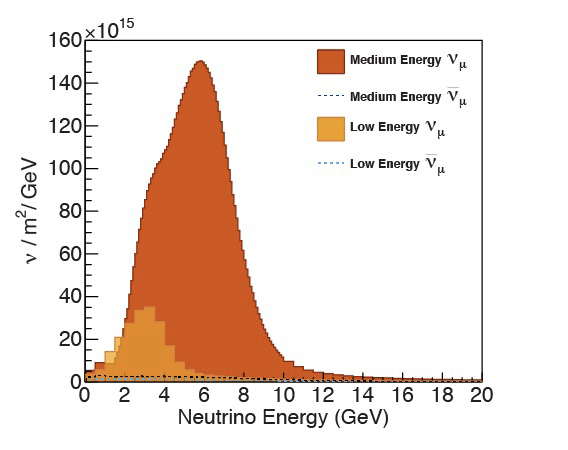
\includegraphics[scale=0.38]{Figures/Chapter2/fluxantineutrino.png}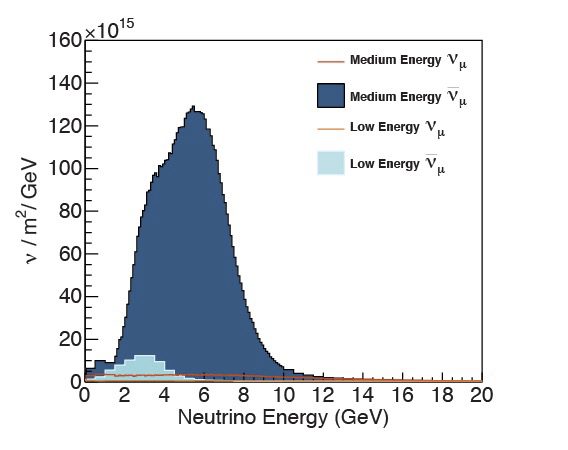
\includegraphics[scale=0.38]{Figures/Chapter2/fluxneutrino.png}
        \caption{Absolute flux for the neutrino mode (left) and the antineutrino mode (right) for the LE and ME eras.} 
\label{fig:MnvExp:NuMI:Flux}
\end{figure}

During the period of 2009 to 2012 the MINER$\nu$A detector collected data in the the Low Energy (LE) mode of the NuMI beam, with a $<E_\nu> = 3$ GeV. For the period of 2013 until 2019 it collected data in the Medium Energy (ME) mode, with a $<E_\nu> = 6$ GeV.  In the \textbf{Figure} \ref{fig:MnvExp:NuMI:Flux}.



\subsection{NuMI Design}

The NuMI beam uses the proton beam produced by the Fermilab Main Injector with an energy of 120 GeV. The proton beam starts accelerating hydrogen ($H^-$) ions using a radio-frequency quadrupole until 750 KeV. In the second stage, the ions are accelerated by a linac from 750 KeV to 400 MeV. The ions are passed through a thin carbon foil to removes the electrons from the $H^-$ obtaining just protons. 

\begin{figure}[!h]
\centering
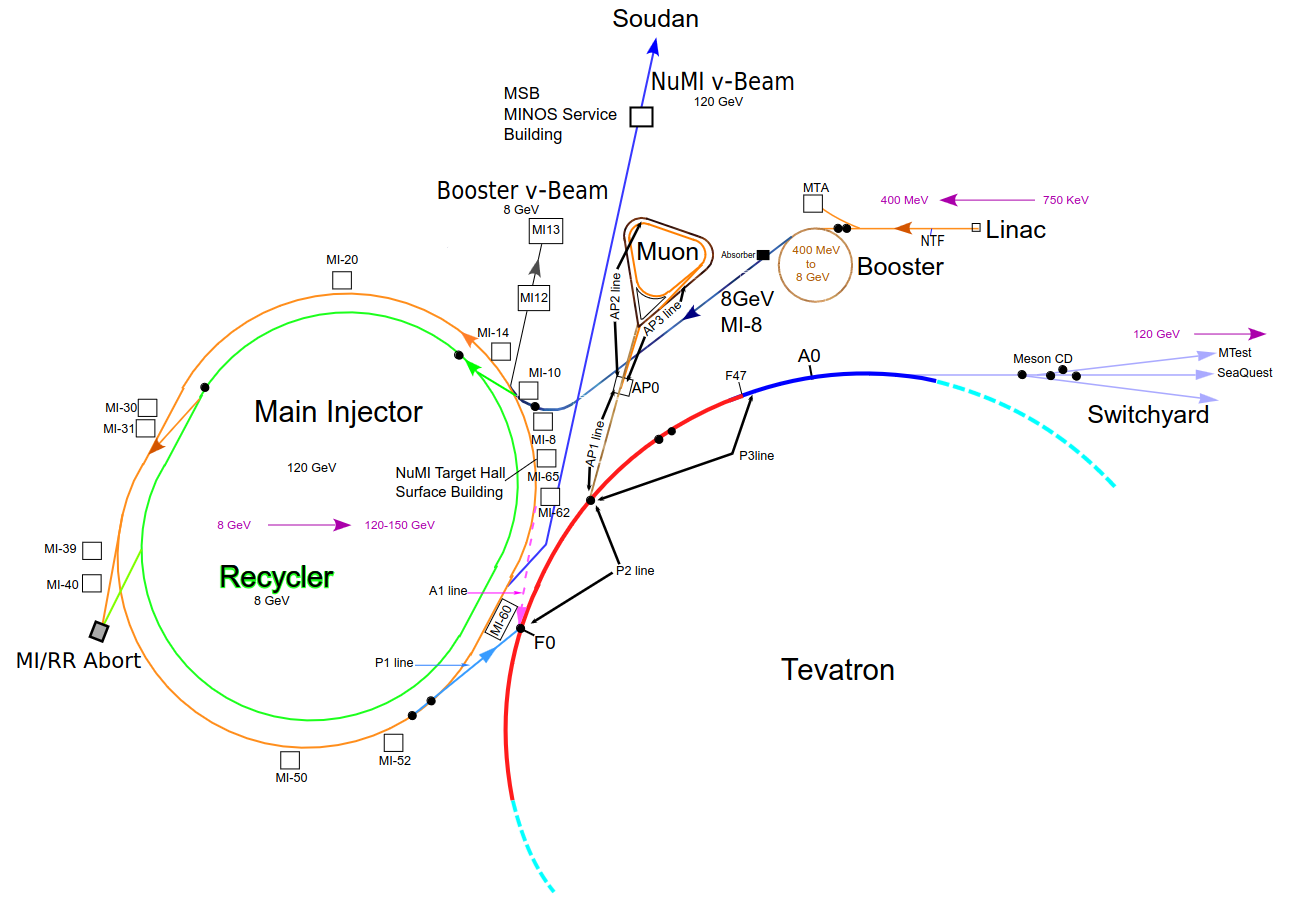
\includegraphics[scale=0.29]{Figures/Chapter2/AcceleratorComplex.png}
        \caption{Schematic of the Fermilab Accelerator complex. Image from \cite{Numi}.} 
\label{fig:MnvExp:NuMI:SchematicMainInjector}
\end{figure}

In the third stage the protons pass to the Booster, it is a 75 m radius synchrotron accelerator that accelerates the protons from 400 MeV to 8 MeV, at the same time it groups the protons in 1.6 $\mu s$ of long batches. 

The last stage of acceleration is on the Main Injector, it is a proton synchrotron 7 times the circumference of the booster. It accelerates the protons from 8 GeV to 120 GeV of energy. The beam produces is has Gaussian shape with a $\sigma =$ 1.1 mm, with a \textit{Cycle Time} = 1.87 s and 10 $\mu s$ beam spill duration. In the  \textbf{Figure} \ref{fig:MnvExp:NuMI:SchematicMainInjector} all the stages of acceleration are shown.

A portion of the proton spills are used by NuMI to produce the neutrino beam, the beam is bent in direction to the NuMI Target Hall. Here the protons are steered to a graphite target. The interaction of the protons with the graphite target produce an hadronical shower where the charged hadrons are focused by two parabolic magnetic horns in direction to the decay pipe. Depending of the current orientation of the current in the pipe, the neutrino mode or antineutrino mode beam can be chosen. The major portion of the hadrons produced are pions and kaons, the predominant decay channel for the pions is $\pi^+ \longrightarrow \mu^+ + \nu_\mu$ and $K^+ \longrightarrow \mu^+ + \nu_\mu$ giving a $\nu_\mu$ beam, for the case of the antineutrino beam, the negative hadrons are focused obtaining as result $\Bar{\nu}_\mu$. 


\begin{figure}[!htb]
\centering
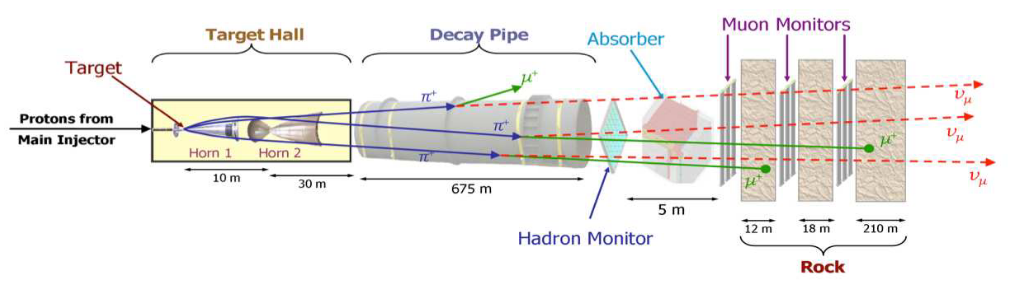
\includegraphics[scale=0.38]{Figures/Chapter2/NuMIScketch.png}
        \caption{Schematic of the Fermilab NuMI Beam. Image from \cite{Numi}.} 
\label{fig:MnvExp:NuMI:SchematicNuMIBeam}
\end{figure}

When the horns focus positive hadrons, the beam consist of 93\% of $\nu_\mu$, 6\% $\Bar{\nu}_\mu$ and 1\% $\nu_e + \Bar{\nu}_e$. In the \textbf{Figure} \ref{fig:MnvExp:NuMI:NuMIBeamComponents} We can observe the different components of the neutrino beam for the neutrino mode in the ME era. 
\begin{figure}[!htb]
\centering
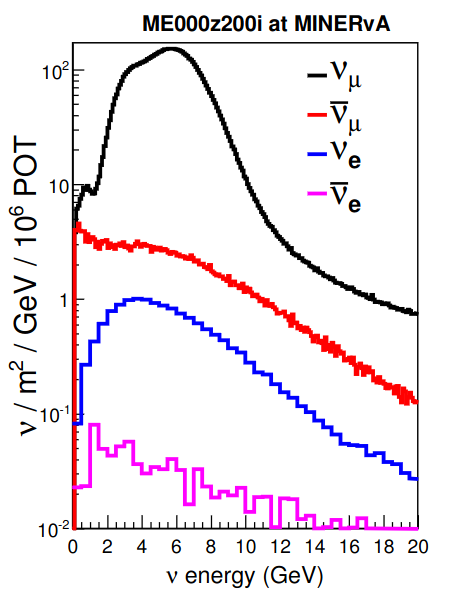
\includegraphics[scale=0.4]{Figures/Chapter2/NuMIbeamComponents.png}
        \caption{Neutrino beam components. Image from \cite{LeoThesis}.} 
\label{fig:MnvExp:NuMI:NuMIviews}
\end{figure}


\subsubsection{NuMI components}
In this subsection, the components of the NuMI beam are described in more detail the components of NuMI.

\textit{NuMI Target Hall}

It is a complex that contains the major part of the components to produce the neutrino beam. In addition to containing a large part of the NuMI instrumentation, it has the roll to shield the high levels of radioactivity, heating and thermal shock that is produced while the beam is on.  

The Target Hall is located in Fermilab approximately 41 m underground, 69 m of length, 8.1 m wide and 12.5 m high. Initially, the beam was designed with the goal to sent neutrinos to MINOS Near (in Fermilab) and Far (in Soudan Laboratory, Minnesota) detectors, therefore, the neutrino beam is bend $3.343^o$ downwards.  

\begin{figure}[!htb]
\centering
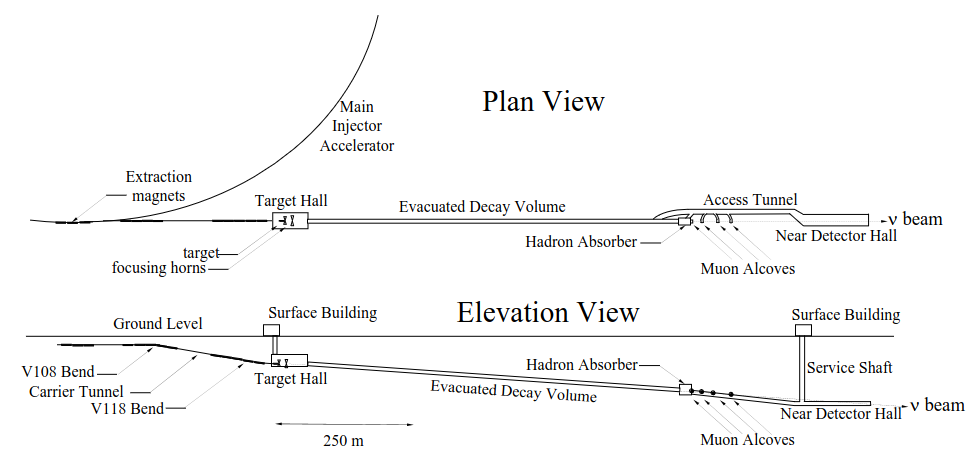
\includegraphics[scale=0.4]{Figures/Chapter2/NuMIFacilityViews.png}
        \caption{Views of the NuMI beam complex. Image from \cite{Numi}.} 
\label{fig:MnvExp:NuMI:NuMIBeamComponents}
\end{figure}

The instrumentation in the Target Hall allows to fix the different beam energy configurations. The energy configuration depends of the distance of between the horns and the target, therefore, it is necessary a central chase. In this chase the components and instrumentation of the beam can be moved depending the beam configuration, at  the same time the chase is also part of the cooling system. 

The cooling system recirculate air in the different components with a capacity of 240 kW of cooling. This system removes the heat for a correct functioning of the beam. For the horns, the cooling system use water to control the temperature.

The NuMI Target Hall has a crane that allow to move, repair and replace equipment remotely. This also has a Work Cell that is a shielded facility where the personnel can access and work in the maintenance of the equipment. 

\textit{The NuMI Target}

The NuMI target is designed to support until 400 kW power without disintegrated, at the same time it should produce the maximizing the production of hadrons and reducing the interactions of the hadrons with the target. So the target can not be very robust because it increase the interaction of the hadrons with the target. The design of the target have to consider that it have to have a high thermal conductivity, it should be available to maintain its mechanical condition at the high temperature conditions, withstand long operational journeys and radiation damage. 

The NuMI Target is made of graphite of type ZXF-5Q with a density of 1.78 g/cm$^3$ \cite{Numi}. It consists of 48 segments of 24 mm long (in beam direction)$\times$ 63 mm tall $\times$ 7.4 mm wide The total length of the target is 95.38 cm, spaced 0.3 mm \cite{BenThesis}.

\begin{figure}[!htb]
\centering
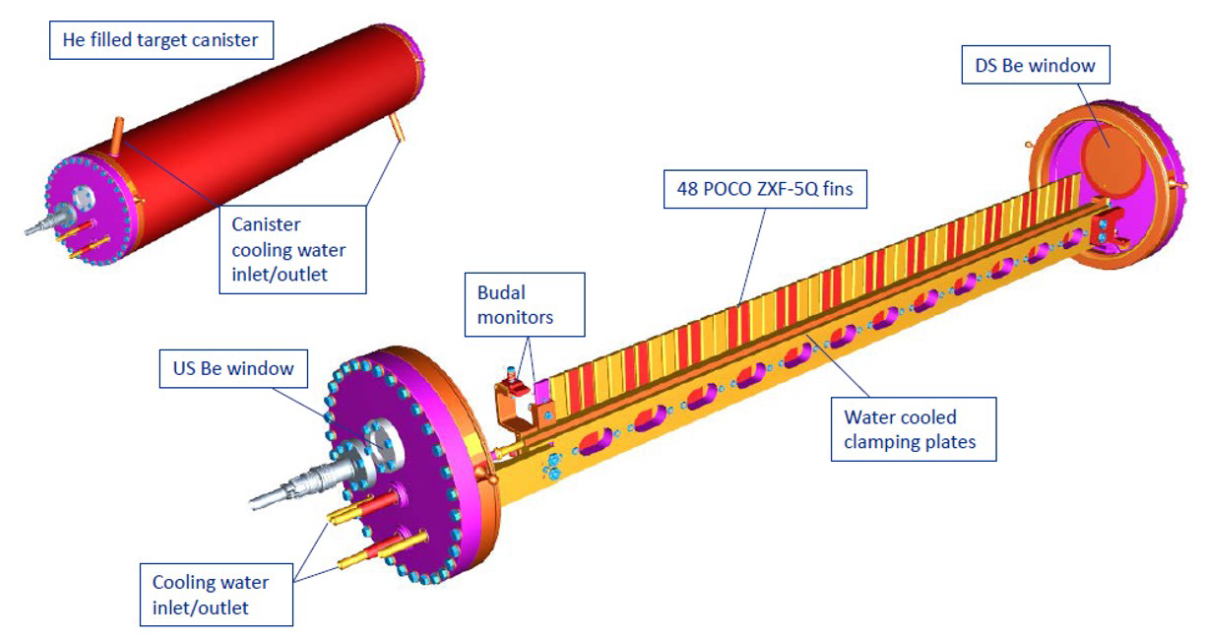
\includegraphics[scale=0.33]{Figures/Chapter2/NuMITarget.png}
        \caption{NuMI Target design for the ME era. Image from \cite{NuMITarget}.} 
\label{fig:MnvExp:NuMI:NuMITarget}
\end{figure}

The NuMI Target is isolated by vacuum and surrounded by two stainless steel tubes that carry the water coolant. These are counted in an aluminum canister filled with He. The entrance and the exit if the beam in the target vessel are made of beryllium. The Budal monitors \cite{Budal} are used to check the alignment of the target respect to the beam. 

\textit{The Target/Baffle Carrier}

The Baffle \cite{NOvATDR} protects the neck of the horn and the cooling hardware form the miss-steered beam pulses. It consist in a 1.5 long graphite core with 57 mm of diameter encased in an aluminum tube. It has an 13 mm diameter center hole along the the rod, where the proton beam passes. 

The Target and the Baffle are mounted in a structure called \textit{Target/Baffle Carrier}. This brings mechanical support, connections to the cooling system and connection to the electrical lines. This structure has installed positioning motors that allow motion of the target vertically and horizontally. 

 \begin{figure}[!htb]
\centering
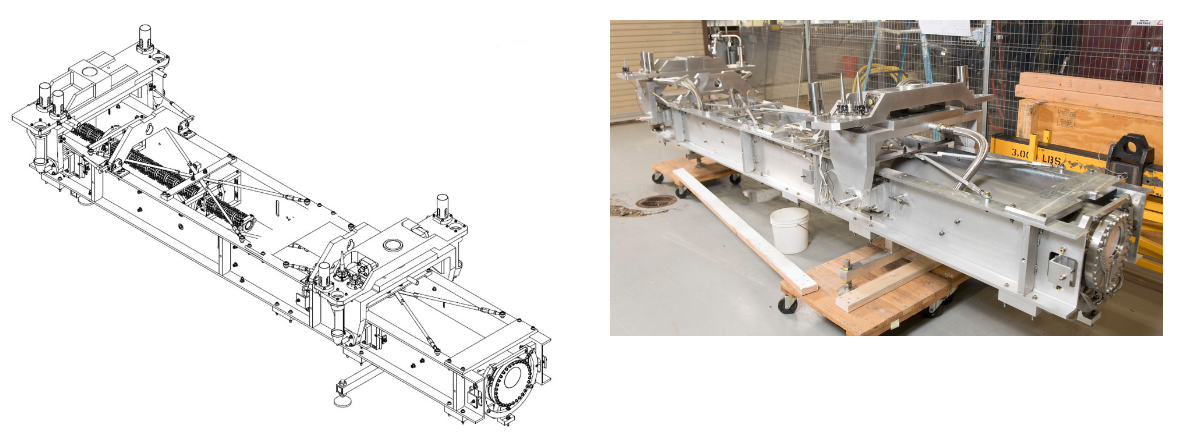
\includegraphics[scale=0.33]{Figures/Chapter2/TargetCarrier.png}
        \caption{Left, NuMI Target/Baffle design. Right, picture of the NuMI Target/Baffle carrier with the target installed. Image from \cite{NuMITarget}.} 
\label{fig:MnvExp:NuMI:NuMITargetCarrier}
\end{figure}

\textit{Magnetic Horns}

The magnetic horns have as their main objective maximize the neutrino flux focusing the secondary particles produced in the target on direction of the detectors, at he same time that can be used to select the neutrino energy spectrum. In the \textbf{Figure} \ref{fig:MnvExp:NuMI:HornsFocusSystem} shows a diagram of how the trajectory of the particles are modified by the horns. 

\begin{figure}[!htb]
\centering
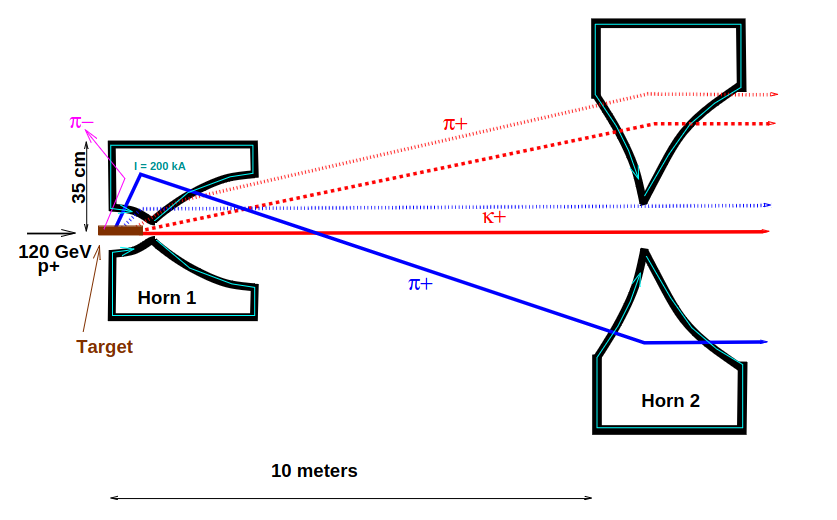
\includegraphics[scale=0.33]{Figures/Chapter2/HornsFocusSystem.png}
        \caption{Schematics of the Horn 1 of Horn 2 modifying the trajectory of the particles. Depending the current direction of the current in the horns the $\nu_\mu$ or $\Bar{\nu}_\mu$ mode can be selected. Image from \cite{Numi}.} 
\label{fig:MnvExp:NuMI:HornsFocusSystem}
\end{figure}

The horns are made of an alloy of nickel-plated aluminum in the inner conductor and for the outer conductor it use anodized aluminum. The inner conductor of the Horn 1 is 2 mm of thickness and 3 mm for the Horn 2 in the most part of the regions. The thickness of the horns should be such that it allows the passage of a large electric current and avoiding the absorption or interaction of the secondary hadrons with the horns. The double paraboloidal shape of the horns produce a toroidal magnetic field where the intensity of the magnetic field falls as the inverse of the radium between the inner and the outer conductors. The expected magnetic field in the longitudinal axis of the horns should be zero and in the maximum transverse field is 3T. To produce the magnetic field in the horns, a pulsed 200 kA of current pass through them with a duration of 2.3 ms.

The high current and the interaction of the hadrons with the horns increases the heat of those, hence, it is necessary to have a cooling system to guaranty a good operation during long periods of time. The cooling system spray water to the inner conductor keeping the temperature below 100 C. 

\begin{figure}[!htb]
\centering
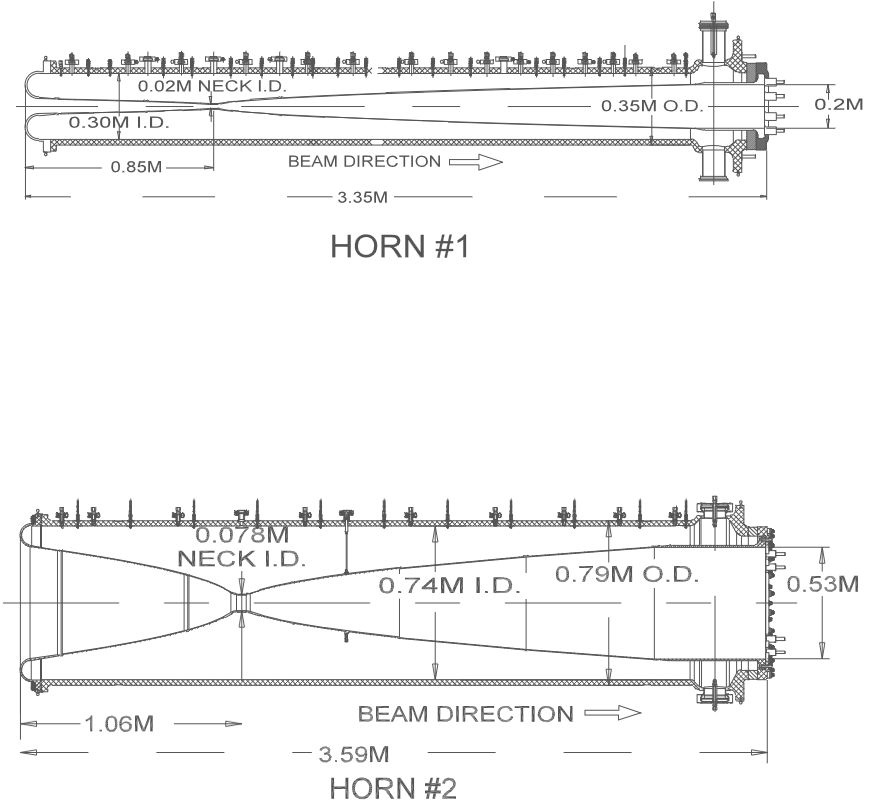
\includegraphics[scale=0.33]{Figures/Chapter2/SchematicMagneticHorns.png}
        \caption{Schematics of the Horn 1 of Horn 2. In the images the dimensions and longitudinal cut of the horns are shown. Image from \cite{Numi}.} 
\label{fig:MnvExp:NuMI:NuMIHornsSchematic}
\end{figure}

Depending of the momentum and the charge of the hadrons, the effects of the horns on the hadrons can be categorized as follow:

\begin{itemize}
    \item \textit{Deflected}: Selecting the direction of the current, the horns can be used to focus only positive or negative hadrons. This allows to select between $\nu$ or $\Bar{\nu}$ beam. It means that when the $\nu$ mode is selected, the negative particles are deflected by the horns, and vise-versa.
    \item \textit{Unfocused} : These are the hadrons that pass very close to the necks of the horns and the trajectory of this particles is not modified by the horns. The most part of these are hadrons with a momentum above to 15 GeV. 
    \item \textit{Underfocused} : These are hadrons that have to pass by the two horns to be focused. The range of the momentum for the hadrons is between 5 GeV and 15 GeV.
    \item \textit{Overfocused}: These are particles that pass throughout the horn 1 and horn 2. Unlike of the underfocused, these are hadrons with a momentum below to the 5 GeV. 
    \item \textit{Horn-1-only}: These are particles that are corrected only by the Horn 1 and that pass throughout the neck of the Horn 2. The transversal momentum of these hadrons usually is above to the 0.2 GeV.
    \item \textit{Horn-2-only} : These are hadrons that pass throughout the neck of the Horn 1 and that are only corrected by the Horn 2. The momentum of these hadrons is between the range of 9 GeV and 15 GeV.
\end{itemize}

\begin{figure}[!htb]
\centering
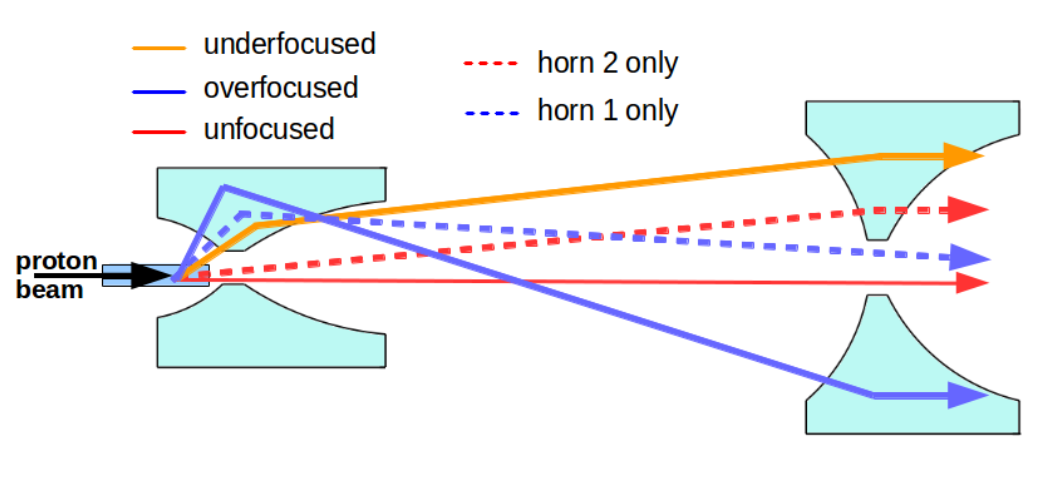
\includegraphics[scale=0.33]{Figures/Chapter2/FocusingComponents.png}
        \caption{Image where the categories of focusing effects are represented. Image from \cite{LeoThesis}.} 
\label{fig:MnvExp:NuMI:NuMIFocusingComponents}
\end{figure}

The focused hadrons with the largest momentum are the hadrons that have a small component of the transversal momentum respect to the proton beam. Therefore, if the horns are close the number of focused hadrons with low momentum increase respect to the high momentum, and vise-versa. Considering this fact, the distance between the horns can be used to select the spectrum energy of the focused hadrons, resulting in a selection of the spectrum of the neutrino beam. The NuMI beam can be used in three energy configurations. Low Energy (LE) where the $<E_\nu>=3.5$ $GeV$, Medium energy (ME) where $<E_\nu>=7$ $GeV$ and High Energy where the $<E_\nu> = 14$ $GeV$\cite{BeamOptics}. 

\begin{figure}[!htb]
\centering
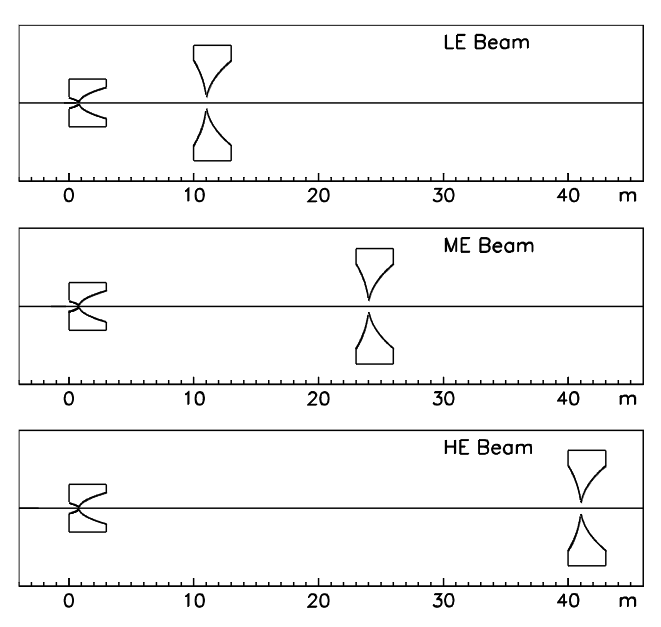
\includegraphics[scale=0.4]{Figures/Chapter2/HornsDistance.png}
        \caption{In this image the distance between the horns for the different energy configurations is shown. Image from \cite{BeamOptics}.} 
\label{fig:MnvExp:NuMI:NuMIFocusingComponents}
\end{figure}

\begin{figure}[!htb]
\centering
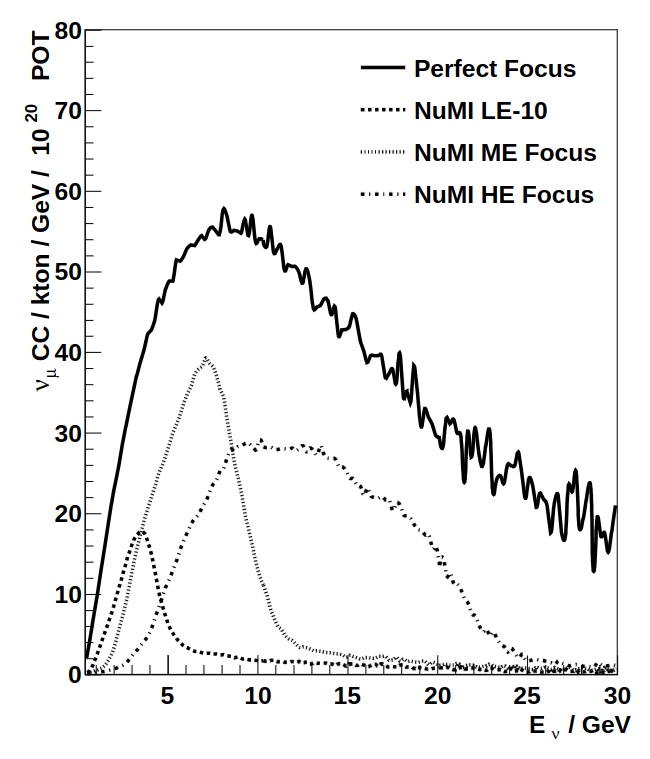
\includegraphics[scale=0.3]{Figures/Chapter2/nuAllSpectrums.png}
        \caption{In this graph, the simulated neutrino spectrum for the different neutrino neutrino energy beam configurations. Image from \cite{Numi}.} 
\label{fig:MnvExp:NuMI:NuMIFocusingComponents}
\end{figure}

\textit{Decay Pipe}

After to focus the secondary hadrons, these pass throughout the \textit{Decay Pipe}. Here, the most part of the hadrons decay and produce the neutrino beam. The goal of the Decay Pipe is to reduce the interactions of the hadrons with the surroundings. To reduce the interactions inside of the Decay Pipe is produced conditions of low density environment. 

The dimensions of the Decay Pipe are 2 m of radius $\times$ 645 m in length. It is surrounded by concrete to reduce the radiation effects in the groundwater. The Decay Pipe is designed to work at internal vacuum conditions and with other low density gases such as helium. 

The collisions of particles with the pipe heat the structure, with the aim to reduce the temperature and to guarantee a long operations of the facility, a cooling system is installed in the pipe. This allow to keep a temperature bellow to the 50 C. 

\textit{Absorber}

Downstream to the Decay Pipe, a structure of aluminum, steel and concrete is installed to stops the protons that did not interact with the NuMI Target and other remnant beam particles, this structure is the absorber. The absorber is an essential component to reduce the levels of radiation and to avoid the groundwater from radiation. The deposition of the energy of the particles generate a temperature increment of the absorber, hence this has a cooling system to maintain the temperature bellow to 50 C. 

\textit{Muon Shield} 

The Muons shield is the last part of the NuMI beam, this works as a shield for the detectors situated in the MINOS Hall from the muons produced in the decay of the mesons in the production of the neutrino beam. This consist in 240 m of dolomite rock that stops the muons. 

\pagebreak



\section{MINER$\nu$A Detector}
\label{Cap:MnvExp:MnvDetector}

The Minerva detector is a fine-grained detector that use as active detection material plastic scintillator to detect the charged particles produced in the neutrino interactions. The design of the detector allows to make a 3D spatial reconstruction at the same time that allows to make a reconstruction of the deposited energy by calorimetric and range techniques. 

The MINER$\nu$A experiment physics goals include produce the measurement of the inclusive and exclusive cross section studies of diverse types of interactions, therefore a good energy reconstruction for low and high energy Final States Interaction (FSI), particle identification and the understanding of multiple interactions in a single beam spill are necessary. Considering the previous points, the detector was design to use different passive nuclear targets, having as active detection material plastics scintillator, that it is a low density active detection material that allows to make a good reconstruction of low energy events. A large portion of the detector is filled of this material with the aim to reconstruct the multi-particle final state at the same time that is surrounded by a electromagnetic (ECAL) and hadronic (HCAL) calorimeters to contain all the particles generated in the interaction. The muons are particles the are not easy to stop, for this reason the detector was situated upstream of the MINOS Near detector with the aim to use it to reconstruct the momentum and determine the charge of the muons produced in the neutrino interactions inside of MINER$\nu$A.


\begin{figure}[!htb]
\centering
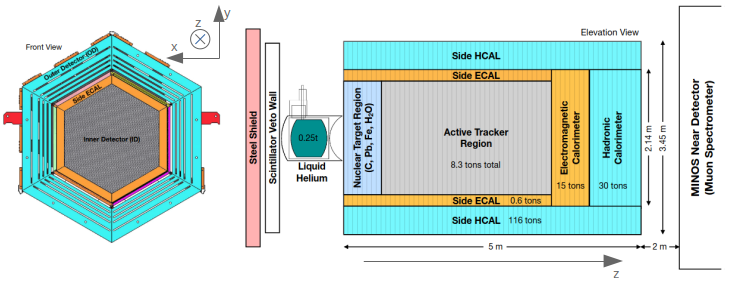
\includegraphics[scale=0.5]{Figures/Chapter2/DetectorScheme.png}

        \caption{Scheme of the MINER$\nu$A detector. . Figure from \cite{ALIAGA2014130}} 
\label{fig:MnvExp:MnvDetector:Scheme}
\end{figure}

The MINER$\nu$A coordinate system is set as follow. The origin of the plane X-Y is situated in the center of the MINER$\nu$A hexagon. The Z axis origin is situated 1200 cm downstream of the MINOS detector, this goes along the center of the MINER$\nu$A detector. The direction of the neutrino beam point 3.34$^o$ downward in the Y-Z plane. 

In the transversal direction of the detector it is segmented in the Inner Detector (ID), where are contained the active tracking planes, nuclear targets, downstream Electromagnetic Calorimeter (ECAL) and the Hadronic Calorimeter (HCAL); and the Outer Detector (OD) that consist of a steel frame with plastic scintillator embedded that works as HCAL and mechanical support to the planes.   

\subsection{Active Tracking planes}
\label{Cap:MnvExp:MnvDetector:ActiveTrackingPlanes}

The detector has active and passive nuclear targets. The active nuclear targets are triangular plastic scintillator strips. When a charge particle pass throughout a scintillator materials, the particle transfers part of its energy to the material, after short time it becomes de-energized emitting light a pulse\cite{DetectionTechniques}. 

The triangular scintillator stripes have a base of 3.3 cm and 1.7 cm height, the length of the strips varies between 85 cm and 170 cm. These are composed of polystyrene doped with  2,5-diphenyloxazol (PPO) and 1,4-bis(5-phenyloxazol-2-yl) benzene (POPOP). These two materials works as weave length shifters. The polystyrene emits light in the far UV region, the PPO absorbs the light en re-emits it in the region of the near UV and then the POPOP absorbs this light and emits it as visible blue light. Along of center of the scintillator strips there is placed an optical fiber that absorbs the blue light and then this re-emits the light on green in the ends of the fiber. The reason for that the light have to be shifted is because the the photo-detectors that transform the light to electrical signals works more efficiently with green light, this process is explained with more detail on the \textbf{subsection} \ref{Cap:MnvExp:MnvDetector:PhotoDetectionSystem}. The scintillator strips are painted with white EJ-510 $TiO_2$ Eljen paint\cite{StripsPaint}. 


\begin{figure}[!htb]
\centering
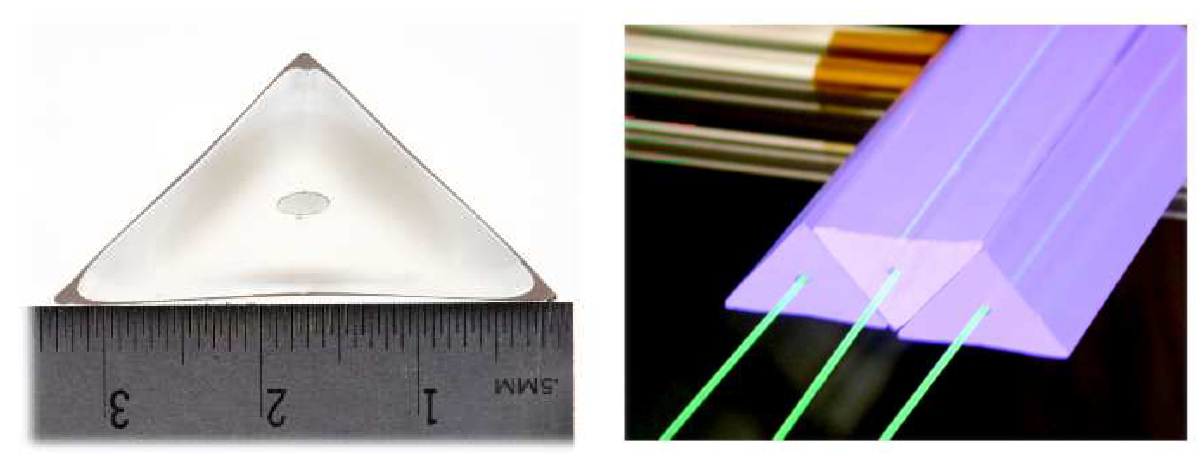
\includegraphics[scale=0.3]{Figures/Chapter2/ScintStripes.png}

        \caption{Images where the plastics scintillators are shown. Figure from \cite{MINERvA}} 
\label{fig:MnvExp:MnvDetector:TriangularStripes}
\end{figure}

The scintillator strips are arranged as is observed in the \textbf{Figure} \ref{fig:MnvExp:MnvDetector:StripsArrange}. The tracking planes are composed of two plastic scintillator planes. On each plane there are 127 strips glued using 3M-DP190 translucent epoxy. The planes are also insulated optically from the exterior. 

\begin{figure}[!htb]
\centering
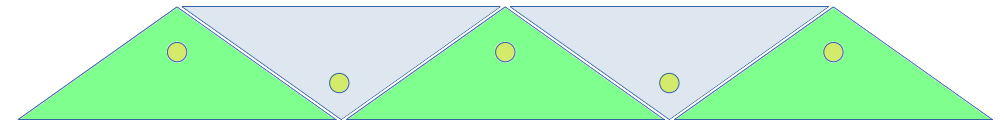
\includegraphics[scale=0.3]{Figures/Chapter2/stripsArrange.png}

        \caption{Scheme that shows how are arranged the scintillator strips to compose the tracking planes.} 
\label{fig:MnvExp:MnvDetector:StripsArrange}
\end{figure}

The tracking planes can be oriented 1 of X, U or V configuration. The orientation of the strips in the X configuration is $90^o$ respect to the horizontal. For the U and V are rotated $60^o$ and $-60^o$ respectively, taking as reference the X orientation, in the \textbf{Figure} \ref{fig:MnvExp:MnvDetector:PlanesOrientations} three schemes of the orientation configurations are shown. The three orientations are used to avoid reconstruction ambiguities for events that contain two particles and deposit energy in orthogonal planes. For the shape and the arrangement of the scintillator strips in the tracking planes, each time that a charge particle pass throughout a plane most part of the particles will interacts with two scintillator strips. 

\begin{figure}[!htb]
\centering
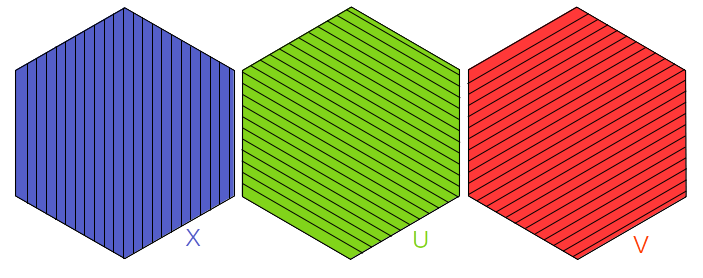
\includegraphics[scale=0.4]{Figures/Chapter2/PlanesOrientation.png}

        \caption{Scheme with that shows the different tracking modules orientations.} 
\label{fig:MnvExp:MnvDetector:PlanesOrientations}
\end{figure}

The planes are grouped in tracking modules, these consist of two tracking planes XU or XV. The modules are stacked in the pattern XUXV, this arrange allows a 3D reconstruction of the charged particles produced by the neutrino interactions that pass through the detector. In the \textbf{Figure} \ref{fig:MnvExp:MnvDetector:TrackingModules} shows a representation of charged particle passing throughout the tracking modules. 

\begin{figure}[!htb]
\centering
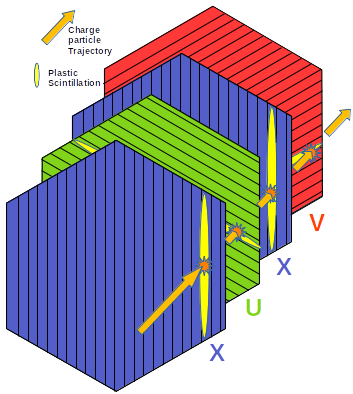
\includegraphics[scale=0.5]{Figures/Chapter2/TrackingModules.png}

        \caption{Scheme where the arrangement of the tracking modules is shown. In the figure is represented how a charged particle produce a signals in the planes.} 
\label{fig:MnvExp:MnvDetector:TrackingModules}
\end{figure}

All the planes are rounded by and hexagonal lead frames that plays the role of ECAL. They are framed by a steel hexagonal frame that bring mechanical support to the hole plane and it is an HCAL. The ECAL and the HCAL that rounds the tracking planes are shown in the \textbf{Figure} \ref{fig:MnvExp:MnvDetector:Scheme}.

\subsection{MINERvA detector Regions}
\label{Cap:MnvExp:MnvDetector:MnvDetectorRegions} 

\begin{itemize}
    \item \textit{Veto wall}

    The Veto Wall is located upstream of the MINER$\nu$A detector, this consist in a steel plate of 5 cm of thickness followed by a plate of plastic scintillator. This section of the detector is used to detect the muons that are produced by the interaction of the neutrino beam with the dolomite rock of the muon absorber. These muons are commonly called \textit{rock muons}.

    \item \textit{Nuclear Targets Region}

    Nuclear Target Region is composed of active and passive targets. The passive materials are Liquid Helium ($He$), Carbon ($C$), Lead ($Pb$), Water ($H_2O$) and Steel ($Fe$). In the \textbf{Figure} \ref{fig:MnvExp:MnvDetector:TargetRegion} the order of how where collocated the planes for passive and active materials in the target region is shown. The C, Pb, $H_2O$ and Fe targets ,in the same way that the active tracking planes, are supported by the ECAL and HCAL.
    
    \begin{figure}[!htb]
    \centering
    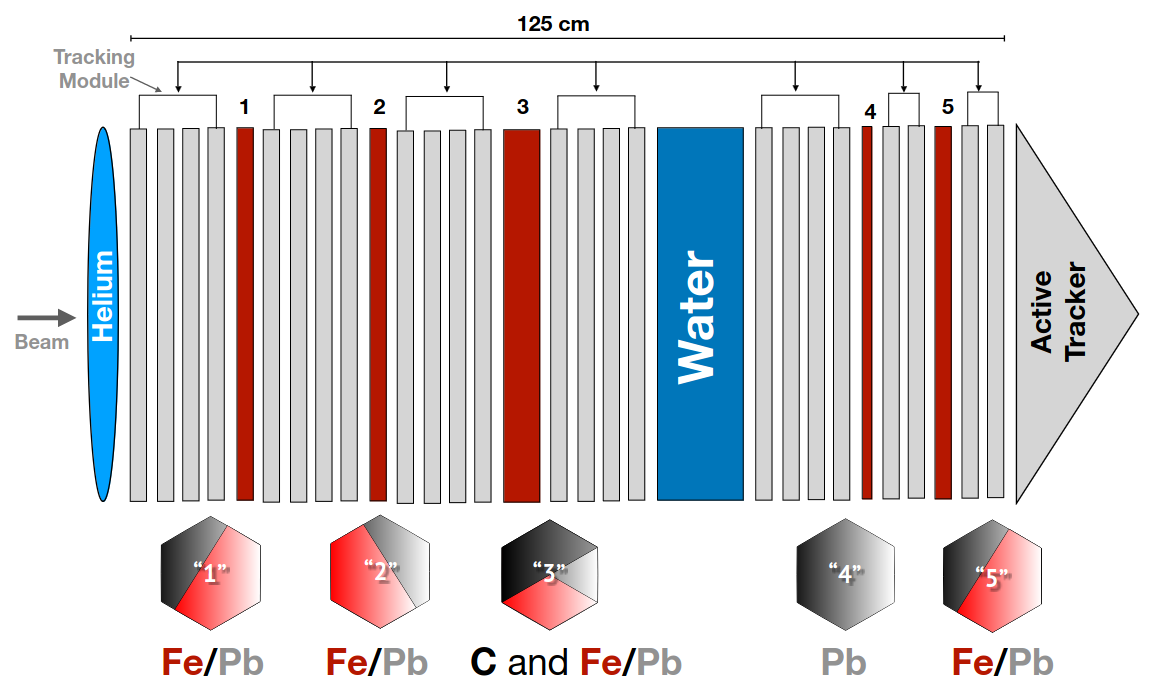
\includegraphics[scale=0.35]{Figures/Chapter2/TargetRegion1.png}

        \caption{Scheme that shows the order that are arranged the target planes in the Target Region. The target region is composed for a cryostat with the Liquid He target, 5 solid targets and the water target. Figure from \cite{MarvinThesis}} 
    \label{fig:MnvExp:MnvDetector:TargetRegion}
    \end{figure}
    
    The He target cryostat is located downstream from the veto wall. This target is capable to contain 2300 L of Liquid He, it was filled during the last parts of the run \cite{ALIAGA2014130}. The other targets are located upstream from the He target. With the aim to localize the neutrino interaction vertex, the nuclear targets planes are located between to tracking modules as shown in the \textbf{Figure} \ref{fig:MnvExp:MnvDetector:TargetRegion}, except for the thin lead target, that only 1 tracking module is located upstream. After the fifth target, the modules of the tracker region starts. In the \textbf{Tables} the information about the composition of the targets is descrived. 

    \begin{table}[!htb]
        \centering
        \begin{tabular}{c c c c c c c c}
            \textbf{Material} & \textbf{Density} & \textbf{C(\%)} & \textbf{Si (\%)} & \textbf{Mn (\%)} & \textbf{Fe (\%)} & \textbf{Cu (\%)} & \textbf{Pb (\%)} \\ 
             & \textbf{(g/cm$^2$)} & & & & & & \\ \hline
            Steel & 7.83±0.03 & 0.13 & 0.2 & 1.0 & 98.7 & - & - \\
            Lead & 11.29±0.03 & - & - & - & - & 0.05 & 99.95\\
            Graphite & 1.74±0.01 & >99.5 & - & - & - & - & - \\ \hline
        \end{tabular}
        \caption{In this table the density and element composition for the solid nuclear targets is shown. Table from \cite{ALIAGA2014130}}.
        \label{tab:Chapter2:Detector:NuclearTargetsComposition}
    \end{table}

    \begin{table}[!htb]
        \centering
        \begin{tabular}{c c c c c c}
            \textbf{Target} & \textbf{z-location} & \textbf{Thickness} & \textbf{Fiducial area} & \textbf{Fiducial mass} & \textbf{Total mass}  \\ 
             & \textbf{(cm)} & \textbf{(cm)} & \textbf{cm$^2$} & \textbf{(kg)} & \textbf{(kg)} \\ \hline
            1-Fe & 452.5 & 2.567±0.006 & 15999 & 322 & 492 \\ 
            1-Pb & 452.5 & 2.578±0.012 & 9029 & 263 & 437 \\
            2-Fe & 470.2 & 2.563±0.006 & 15999 & 321 & 492 \\ 
            2-Pb & 470.2 & 	2.581±0.016 & 9029 & 263 & 437 \\
            3-Fe & 492.3 & 	2.573±0.004 & 7858 & 158 & 238 \\ 
            3-Pb & 492.3 & 2.563±0.004 & 3694 & 107 & 170 \\
            3-C & 492.3 & 7.620±0.005 & 12027 & 160 & 258 \\ 
            Water & 528.4 & 17–24 & 25028 & 452 & 627 \\
            4-Pb & 564.5 & 0.795±0.005 & 25028 & 225 & 340 \\
            5-Fe & 577.8 & 1.289±0.006 & 15999 & 162 & 227 \\ 
            5-Pb & 577.8 & 1.317±0.007 & 9029 & 134 & 204 \\ \hline
        \end{tabular}
        \caption{The z position, thickness, fiducial area, fiducial mass and total mass of the nuclear targets are shown. The z-location is determined according the coordinate system described in the text. Table from \cite{ALIAGA2014130}. }
        \label{tab:Chapter2:Detector:Sizes}
    \end{table}

    The water target, unlike the solid targets, is hold by a circular frame. The diameter of this frame is larger that the MINER$\nu$A inner detector size. The water container is made of two Kevlar\textsuperscript \textregistered sheets. The internal hydrostatic pressure of water deform the shape of the water container, for that reason the water target is not well defined. The geometry of the targets is part of the parameters of the particle simulation it is necessary to have a good  approximation of the shape of the targets, with the aim to obtain the best approximation to the water target shape, the container shape was simulated via finite element analysis. 

    \begin{figure}[!htb]
        \centering
        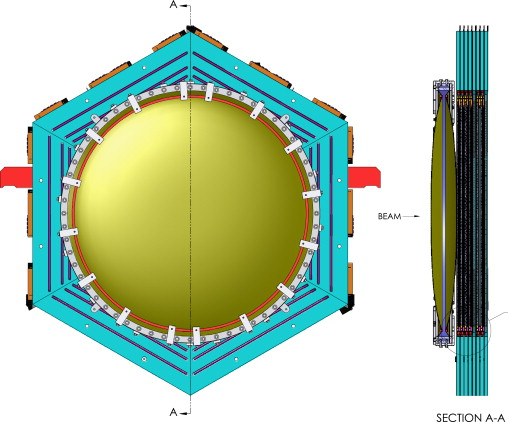
\includegraphics[scale=0.6]{Figures/Chapter2/WaterTarget.jpg}
        \caption{Scheme of the water target. Image from \cite{ALIAGA2014130}.}
        \label{fig:MnvExp:MnvDetector:WaterTarget}
    \end{figure}

    
    \item \textit{Active Tracker Region}
    
    The active tracker region consist of 61 tracker modules, giving a total of 122 tracking planes. This region the ID volume is filled completely of plastic scintillator, described in \ref{Cap:MnvExp:MnvDetector:ActiveTrackingPlanes}, and the OD volume consist of the ECAL and HCAL.
    
    \item \textit{Electromagnetic and Hadronic Calorimeter modules}
    
    The ID ECAL is located upstream the tracker region. The configuration of the planes in the ECAL region is similar to the tracker region, except that each plane has a 0.2 cm thick layer of lead embedded to the upstream side of the plane. This layer helps to stops the electrons and photons produced in the interaction vertex, obtaining a good energy resolution and directional information. This region contains 10 of this modules. 

    For the case of the ID HCAL, it has a similar configuration that the tracker region, but it has an steel plane of 2.54 cm thick each two planes, that is, each module has one steel plane. In the same way that the ECAL but with heavier particles, it allow a good energy resolution and directional information of particles such as protons and neutrons. 
    
\end{itemize}

\subsection{MINOS Near Detector}
\label{Cap:MnvExp:MnvDetector:MINOS}

The MINER$\nu$A detector is situated 2.1 m from the MINOS Detector and is used by MINER$\nu$A as muon spectrometer. The MINOS Near detector is designed to measure the muon neutrino flux close to the NuMI beam, performing a precise measurement in neutrino oscillation parameters for the muon neutrino disappearance. The MINOS Near detector is a magnetized tracking calorimeter composed of planes of plastic scintillator an iron giving a total mass of 1 kTon \cite{MINOSpaper}. The rectangular coil produce a toroidal magnetic field of a average strength of 1.3 T.

\begin{figure}
    \centering
    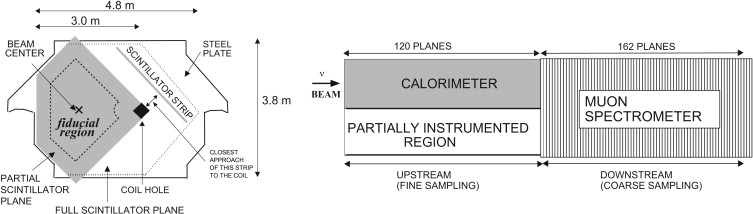
\includegraphics[scale=0.9]{Figures/Chapter2/MINOSNDScheme.jpg}
    \caption{Scheme of the lateral and frontal view of the MINOS Near detector. Some of the main components of the detector are shown. Figure from \cite{ALIAGA2014130}.}
    \label{fig:MnvExp:MnvDetector:SchemeMINOSND}
\end{figure}

The MINOS detector is able to measure the energy of the muon by the curvature or by range. The reconstruction by range is applied when the muon is contained in the detector measuring the ionization energy in the plastic scintillator and adding the correction for the passive steel. For the cases where the muon is not contained in the detector, the energy is reconstructed by the curvature of the track of the muon deflected by the magnetic field in MINOS. The energy measured by range is more precise that by curvature, for that it is preferred in the case that it is reconstructed by the two methods. For the reconstruction of the total muon energy, the energy measured by MINOS is added to the deposited energy of the muon in MINER$\nu$A. 


\begin{figure}[!htb]
    \centering
    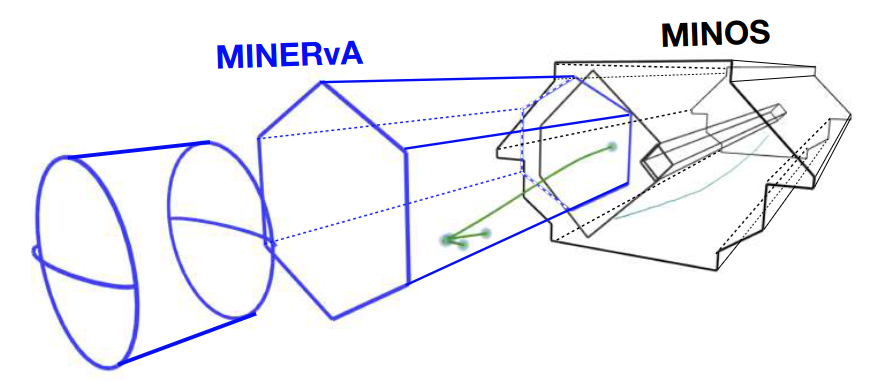
\includegraphics[scale=0.4]{Figures/Chapter2/MnvMINOS.png}
    \caption{Scheme that shows the volume of the He target, ID volume and the MINOS detector. In the scheme is shown how the MINER$\nu$A detector is aligned to the fiducial region of the MINOS detector. Image from \cite{MarvinThesis}.}
    \label{fig:MnvExp:MnvDetector:WholeMINERvADet}
\end{figure}

\subsection{Photodetection System}
\label{Cap:MnvExp:MnvDetector:PhotoDetectionSystem}

The light produced in the scintillator is downshifted by a wavelength shifting (WLS) fiber that is located in the center of the scintillator strip. The end of this fiber is polished to mirror level. The end of the cables are encrusted to optical connectors from Fujikura-DDK \cite{OpticalConnector}. Each connector holds 8 fibers in a linear shape. The connectors are referred to the other DDK connector, this connector holds 8 clear polished fibers. This cables transmit the light from the WLS to the photo-multipliers (PMT) boxes. All the WSL were tested checking the attenuation at different distances of the fiber and for the clear fibers were tested measuring the transmission of light. These procedures are described in \cite{ALIAGA2014130}.

\begin{figure}[!htb]
    \centering
    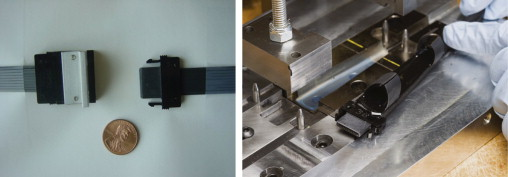
\includegraphics{Figures/Chapter2/OpticCablesConnectors.jpg}
    \caption{In the left, picture of the DDK connector. In the right the process of attach of the optical wires to the DDK connectors. Figure from \cite{ALIAGA2014130}.}
    \label{fig:MnvExp:MnvDetector:DDKConnector}
\end{figure}

The optical box consists in a frame that contains the Fiber-end Face plate, the cookie, the PMT, FEB connector board, two imputs for the Light Injection (LI) system, connecting cables and the Optical Decoder Unit (ODU). The ODU is an array that connects the Fiber-end face plate to the PMT. In the \textbf{Figure} \ref{fig:MnvExp:MnvDetector:OpticalBox} the components of the Optical box are shown. 

\begin{figure}[!htb]
    \centering
    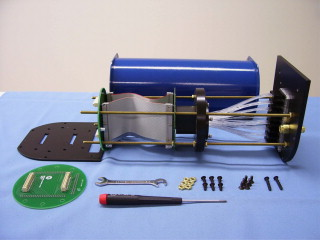
\includegraphics{Figures/Chapter2/OpticaBox.jpg}
    \caption{Picture where the internal components of the optical box. Figure from \cite{ALIAGA2014130}.}
    \label{fig:MnvExp:MnvDetector:OpticalBox}
\end{figure}

The photo-multipliers, more commonly known as PMTs, are sensitive light detectors that transform the light that is collected by the sensitive region in to an electric signal. The physics beyond the PMT is based on the photo-electric effect, when the photons pass through the input window and interacts with a  cathode it produce photo-electrons, these are accelerated by an electric field produced by a dynodes chain where the electrons collide producing a positve gain in the number of electrons. This technology allows to have information of the initial number of photons given the multiplicative factor of charge, the size of the signal is related with the deposited energy of the particles on the scintillator. 

\begin{figure}[!htb]
    \centering
    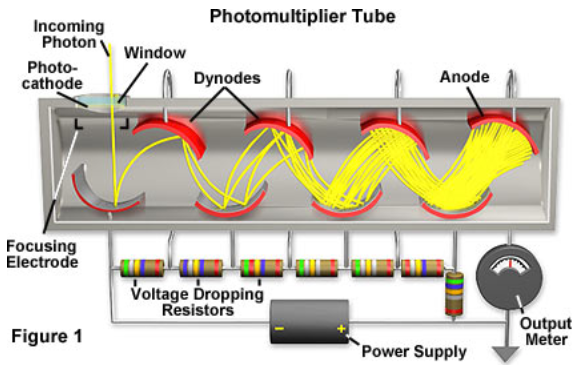
\includegraphics[scale=0.5]{Figures/Chapter2/PMT.png}
    \caption{Scheme where the functionality of a PMT is shown. In the image the mainly components of a PMT are shown. Figure from \cite{PMTHamamatsu}.}
    \label{fig:MnvExp:MnvDetector:PMTfunctionality}
\end{figure}



The PMT's model used is H8804MOD-2 manufactured by Hamamatsu Photonics \cite{hamamatsu2007photomultiplier}. The H8804MOD-2 PMT has an 8$\times$8 matrix of 2 mm $\times$ 2 mm pixels, giving a total of 64 pixels. The quantum efficiency required is 12\% at 520 nm and a maximum-to-minimum pixel gain  The spectral response of the PMT is 300-650 nm.    

The ODU has as main goal to separate physically the signal from adjacent scintillator strips, in the way that these are not adjacent pixels in the PMT. This distribution helps to reduce the cross-talk efects that can be presented in the plastic bars. In the \textbf{Figure} \ref{fig:MnvExp:MnvDetector:ODU} a diagram of the fibers pater is shown. 

\begin{figure}[!htb]
    \centering
    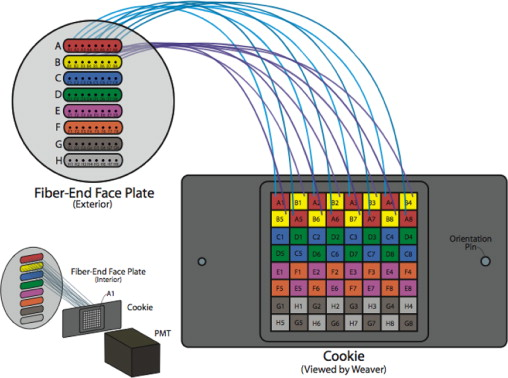
\includegraphics{Figures/Chapter2/ODU.jpg}
    \caption{Pattern of distribution of the fibers for each PMT. Figure from \cite{ALIAGA2014130}.}
    \label{fig:MnvExp:MnvDetector:ODU}
\end{figure}

Each optical box has two inputs for the light injection system (LI). This system consist in a light box that produce a blue pulsed light that is sent by two clear optical cables to each optical boxes, inside of the optical boxes the light is distributed uniformly over all the PMT pixels. The LI system turns on during ones after each beam spill. In this test the gain of the PMTs is measured and is used to monitoring the gain of the PMTs dearly. 

The output of the PMTs are connected to an electronic board know as front-end board (FEB). This electronic board digitize the analogical height and timing pulse that comes from the PMTs, provides a high voltage (HV) to the PMT and it send the digitized information to the Data Acquisition System (DAQ). 

\begin{figure}
    \centering
    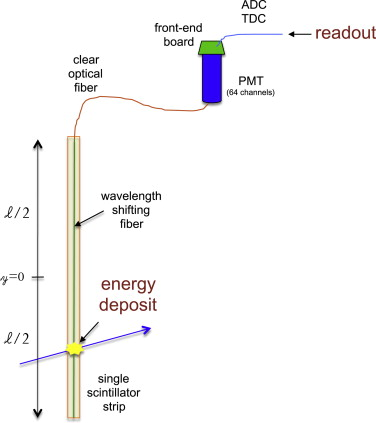
\includegraphics{Figures/Chapter2/OpticalSystem.jpg}
    \caption{Scheme that shows the meanly components of the optical system. It shows how the light travels from the plastic scintillator strips to the optical box. Figure from \cite{ALIAGA2014130}.}
    \label{fig:enter-label}
\end{figure}

\subsection{Calibration}
\label{Cap:MnvExp:MnvDetector:Calibration}

\subsection{Data Reconstruction}
\label{Cap:MnvExp:MnvDetector:DataReconstruction}

\subsection{Data Acquisition System }
\label{Cap:MnvExp:MnvDetector:DAQ}

The Data Acquisition System has a main roll collect all the information generated in the neutrino interaction and save it. 

After that the light is produced in the plastic scintillator strips, is explained in the \textbf{Subsection} \ref{Cap:MnvExp:MnvDetector:ActiveTrackingPlanes}, the light is carried by the 








	\chapter{Simulation}
\minitoc
\label{Cap:Simulation}

\section{Introduction}
\label{Cap:Simulation:Introduction}
The simulation of the MINER$\nu$A detector has multiple functions, such as background estimation, efficiency detector studies, simulation of reconstruction and the comparison of different  model with data. In this Chapter the different steps of the MINER$\nu$A experiment simulation are explained, including the beam simulation and a brief description of the models used by the simulators.

The simulation starts with the beam simulation, followed by the neutrino interaction simulation inside of the MINER$\nu$A detector geometry. It proceeds with the simulation of the propagation of the resultant particles in the interaction with the detector, here the deposited energy, the particles track and secondary particles are simulated. The last part of the simulation consist in a decalibration of the results from the previews stage in the way to simulate the same conditions of the real detector. At the end, it returns the simulated data in the same format that the raw data. In the following sections, the simulation steps are explained.

\section{Beam simulation}
\label{Cap:Simulation:BeamSimulation}

The neutrino flux simulation is performed in G4NuMI, based in GEANT 4 \cite{GEANT4}. In this stage the production of hadrons, the focusing and the secondary interactions of the hadrons with the different components of NuMI are simulated. It starts giving as input the proton beam from Main Injector and finishes with the neutrino beam. A detailed description of the flux simulation can be found here \cite{LeoThesis}.

Most part of NuMI geometry components are included in the simulation, such as the magnetic horns, the decay pipe, the absorbers, etc. The flux simulation is specially sensitive to the hadron production and the flux focusing. 

The proton beam from Main Injector, it corresponds to a 120 GeV kinetic energy with a Gaussian transverse profile distribution with $\sigma$ = 1.1 mm, continuing with the hadron production simulation. For the hadron production, the GEANT 4 hadronic model by the fault use the  




\section{Interaction Simulation}
\label{Cap:Simulation:InteractionSimulation}

\subsection{GENIE}
\label{Cap:Simulation:GENIE}

\section{Detector Simulation}
\label{Cap:Simulation:DetectorSimulation}

\subsection{GEAN 4}
\label{Cap:Simulation:GEANT4}

\section{MC reconstruction}
\label{Cap:Simulation:MCReconstruction}





	\chapter{Analysis}
\minitoc
\label{Cap:Analysis}
%++++++++++++++++++++++++++++++++++++++
%     Introduction 
%++++++++++++++++++++++++++++++++++++++

\section{Introduction}
\label{Cap:Analysis:Introduction}
In the \textbf{Subsection} \ref{Cap:Int:Motivation} In this thesis are presented the results for a differential cross section (1D cross section) and a double differential cross section (2D cross section). The signal definition for both is the same. 

%++++++++++++++++++++++++++++++++++++++
%     Signal definition 
%++++++++++++++++++++++++++++++++++++++

\section{Signal Definition}

%++++++++++++++++++++++++++++++++++++++
%     Data Selection 
%++++++++++++++++++++++++++++++++++++++
\section{Data Selection}



%++++++++++++++++++++++++++++++++++++++
%     Background Sustraction
%++++++++++++++++++++++++++++++++++++++
\section{Background studies}

\subsection{Background tuning}

\subsection{Background subtraction}

%++++++++++++++++++++++++++++++++++++++
%     Migration Matrix
%++++++++++++++++++++++++++++++++++++++
\section{Migration Matrix}


%++++++++++++++++++++++++++++++++++++++
%     Ungolding
%++++++++++++++++++++++++++++++++++++++

\section{Unfolding}

\subsection{Warping Studies}

\subsection{Unfolded Distributions}

%++++++++++++++++++++++++++++++++++++++
%     Efficiency  
%++++++++++++++++++++++++++++++++++++++

\section{Efficiency}

\subsection{Efficiency correction}

	\chapter{Cross Section Results}
\minitoc
\label{Cap:xSec}

The results of the cross section measurement are presented in this chapter. The measurements report both statistical and systematic errors. The systematic errors are detailed in \textbf{Chapter} \ref{Cap:ErrorAnalysis}. Some details and observations are given in the \textbf{Sections} \ref{Cap:xSec:1DResults} and \ref{Cap:xSec:2DResults}.

\section{Single differential Cross Section Results}
\label{Cap:xSec:1DResults}

For $E_\nu$, see \textbf{Figure} \ref{fig:Analysis:CrossSection:1DCrossSectionenu}, it is observed that the prediction and data are well matched in most parts of the bins. This is because most of the neutrino energy reconstruction comes from the muon momentum, which is generally well reconstructed because of the MINOS Near detector. However, the hadronical energy is biased for multiple reasons, which are considered in the systematic error calculation.  

$T_\pi$, \textbf{Figure} \ref{fig:Analysis:CrossSection:1DCrossSectionmixtpi}, does not match perfectly in most parts of the bins. The first two bins correspond to a region never reported in previous analyses. The good match between the data and the MC for the first two bins is also related to the effects of the pion reweight. The larger disagreement between the data and the simulation is observed in the fourth bin, where the data point is more than 1$\sigma$ far from the simulation.

Something that must be considered for the results of $\theta_\pi$, \textbf{Figure} \ref{fig:Analysis:CrossSection:1DCrossSectionmixthetapi_deg}, is the different signal definition in which the kinetic energy of the pion is limited between 20 MeV and 350 MeV. The MC histograms correspond to the GENIE 2.12.6 event generator, re-weighted by the MINER$\nu$A weight MnvGENIE v4.3.1 + Pion re-weight, as explained in \textbf{Chapter} \ref{Cap:Simulation:GENIE}. In the case of $\theta_\pi$, there is observed a disagreement between the data and the simulation. The shape of the distribution is similar. The higher change of the cross section is located around 90 degrees. It is observed that the cross section is not symmetric with respect to 90 degrees. 

$P_\mu$, see \textbf{Figure} \ref{fig:Analysis:CrossSection:1DCrossSectionpmu}, has good agreement between the data and the simulation. This is related to the good reconstruction of the muon kinematics and the fact that most of the neutrino energy is taken by the lepton, in this case a muon.

$P^t_\mu$, see \textbf{Figure} \ref{fig:Analysis:CrossSection:1DCrossSectionptmu}, has good agreement between the shape and central value of the data and the simulation. The central values are statistically compatible in most of the bins. 

$P^z_\mu$, see \textbf{Figure} \ref{fig:Analysis:CrossSection:1DCrossSectionpzmu}, also shows a good agreement between the data and simulation. The peak of the cross section for the simulation is observed more to the right of the data point; however, the central values are statistically compatible. 

$\theta_\mu$, see \textbf{Figure} \ref{fig:Analysis:CrossSection:1DCrossSectionthetamu_deg}, has good agreement between the data and the simulation. The shape of the cross sections are very similar, and the largest discrepancy is observed in the last three bins. 

In $Q^2$, see \textbf{Figure} \ref{fig:Analysis:CrossSection:1DCrossSectionthetamu_deg}, the disagreement between the data and the MC increases in the low $Q^2$ region. This has also been reported in other analyses, such as \cite{Bercellie.131.011801} and \cite{Eberly:2014mra}. The shape is similar and the maximum distribution is observed in the same region.

The cross section reported here $W_{exp}$, see \textbf{Figure} \ref{fig:Analysis:CrossSection:1DCrossSectionwexp}, is highly dependent on the reconstructed $E_{had}$. This variable is not easily reconstructed because of the smearing effect caused by neutral particles, which are not observed directly in the detector. It is also highly dependent on interactions inside the nucleus, which are not directly measured, also. All these effects are included in the systematic errors. The maximum observed between the bin edges 1200 MeV and 1300 MeV corresponds well to the $\Delta$ (1232) production. The results for this variable are not very reliable due to the findings of the warping studies, where the variable demonstrates that it cannot unfold.


\foreach \var in  {enu,mixtpi,mixthetapi_deg,pmu,ptmu,pzmu,thetamu_deg,q2,wexp}{
%\foreach \var in  {enu_true,mixtpi_true,pmu_true,ptmu_true,pzmu_true,thetamu_deg_true,q2_true,wexp_true}{
    \ifthenelse{\equal{\var}{enu}}{
      \renewcommand{\NewVar}{E_\nu}
    }{}
    \ifthenelse{\equal{\var}{mixtpi}}{
      \renewcommand{\NewVar}{T_\pi}
    }{}
    \ifthenelse{\equal{\var}{mixthetapi_deg}}{
      \renewcommand{\NewVar}{\theta_\pi}
    }{}
    \ifthenelse{\equal{\var}{pmu}}{
      \renewcommand{\NewVar}{P_\mu}
    }{}
    \ifthenelse{\equal{\var}{ptmu}}{
      \renewcommand{\NewVar}{P^T_\mu}
    }{}
    \ifthenelse{\equal{\var}{pzmu}}{
      \renewcommand{\NewVar}{P^z_\mu}
    }{}
    \ifthenelse{\equal{\var}{thetamu_deg}}{
      \renewcommand{\NewVar}{\theta_\mu}
    }{}
    \ifthenelse{\equal{\var}{q2}}{
      \renewcommand{\NewVar}{Q^2}
    }{}
    \ifthenelse{\equal{\var}{wexp}}{
      \renewcommand{\NewVar}{W_{exp}}
    }{}
    \begin{figure}
        \centering
        \includegraphics[scale=0.3]{Figures/Chapter5/CrossSection/CrossSection_\var__1Pi_BWN.png}
        \caption{$\NewVar$ 1D Cross Section. Figure by the author.}
        \label{fig:Analysis:CrossSection:1DCrossSection\var}
    \end{figure}  
}

The bigger discrepancies between the models and the data are observed in the variables that have a larger dependency on the nonmuon variables. For variables such as $Q^2$, $E_\nu$ and $W_{exp}$ requires a good measurement of the hadronic energy, which depends on a good reconstruction of charged and neutral particles, with neutral particles being especially difficult to measure. For future measurements, it is necessary to have a better estimation of the hadronic energy adding the estimated energy of neutrons.

For the reconstruction of $T_\pi$, it is necessary to have a better description of how the pions interact with the detector, especially for pions with an energy greater than 200 MeV. The $T_\pi$ weight provides a better prediction of the high and low $T_\pi$ region, see \textbf{Figure} \ref{fig:Analysis:Cuts:DataSelBreakdownTpireweight}, but lacks a physics-based explanation. Hence, it is necessary to compare with other models to have a deeper understanding about what is modulating the predictions in those regions. 

Other variables that can be added to this analysis are the Adler angles \cite{S_nchez_2016}. These variables allow to take as reference system the nucleus and as Z axis the hadronic momentum. These variables provide information about the nuclear effects, which are of great importance for modeling nuclear dynamics for a massive nucleus.  

There are other neutrino interaction MC generators that can be used to simulate the cross section such as NuWro \cite{juszczak2009runningnuwro}, GiBUU \cite{GiBUU}, GENIE v3 \cite{GENIE:2021npt}, etc.


\pagebreak

\section{Two Differential Cross Section Results}
\label{Cap:xSec:2DResults}

As explained in the introduction of the Chapter \ref{Cap:Analysis:Introduction}, the two differential cross section results do not include the untracked pions, and the kinetic energy is restricted for the range from 35 MeV to 350 MeV. The event generator used for this analysis is also GENIE 2.12.6 re-weighted by MnvGENIE v4.3.1, this is described in the \textbf{Chapter} \ref{Cap:Simulation:GENIE}. 

For the combination of $P^t_\mu$ and $T_\pi$, see \textbf{Figures} \ref{fig:Analysis:CrossSection:2DEfficiencyptmu_vs_tpi} and \ref{fig:Analysis:CrossSection:2DEfficiencytpi_vs_ptmu}, the simulation overestimates the cross section value for values of high $T_\pi$. For most of the other bins, the simulation and data are statistically consistent. The disagreement in the last bin can be explained as an effect of a lack of understanding of the inelastic interactions of pions with the detector.


The results for the combination of $P^T_\mu$ and $P^z_\mu$, see \textbf{Figures} \ref{fig:Analysis:CrossSection:2DEfficiencyptmu_vs_pzmu} and \ref{fig:Analysis:CrossSection:2DEfficiencypzmu_vs_ptmu}, generally show good agreement between the data and the simulation, even for bins with low statistics. 

$P_\mu$ and $T_\pi$, see \textbf{Figure} \ref{fig:Analysis:CrossSection:2DEfficiencytpi_vs_pmu} and \ref{fig:Analysis:CrossSection:2DEfficiencypmu_vs_tpi}, generally show good agreement between the data and the simulation. As observed in the other combinations with $T_\pi$, at high $T_\pi$ the simulation overestimates the cross section.  


The cases of $T_\pi$ and $\theta_\pi$, see \textbf{Figures} \ref{fig:Analysis:CrossSection:2DEfficiencythetapi_deg_vs_tpi} and \ref{fig:Analysis:CrossSection:2DEfficiencytpi_vs_thetapi_deg},  are not reliable, similar to the case of $W_{exp}$ in single differential cross sections, this combination of variables cannot be unfolded. However, it can be observed that at high $T_\pi$ the data and the simulations do not agree well. In the same way, the pions that travel backward are underestimated. 

$T_\pi$ and $E_\nu$ combinations, see \textbf{Figures} \ref{fig:Analysis:CrossSection:2DEfficiencyenu_vs_tpi} and \ref{fig:Analysis:CrossSection:2DEfficiencytpi_vs_enu}, show a good agreement between the data and the simulation. The high $T_\pi$ also shows that the simulation overestimates the cross section. The goal of the combinations of these two variables is to compare the cross sections with the previous single pion production analysis produced in MINER$\nu$A for the LE and ME eras.

Something that should be highlighted from this study is that it is the first 2D analysis in MINER$\nu$A collaboration that shows the cross section as a function of hadronic variables, such as $T_\pi$ and $\theta_\pi$.

%\foreach \var in {loW,midW,hiW}{ 
\foreach \var in  {ptmu_vs_tpi,tpi_vs_ptmu,ptmu_vs_pzmu,pzmu_vs_ptmu,tpi_vs_pmu,pmu_vs_tpi,thetapi_deg_vs_tpi,tpi_vs_thetapi_deg,enu_vs_tpi,tpi_vs_enu}{


    \ifthenelse{\equal{\var}{pzmu_vs_ptmu}}{
      \renewcommand{\NewVar}{P^z_\mu,P^T\mu}
    }{}
    \ifthenelse{\equal{\var}{tpi_vs_thetapi_deg}}{
      \renewcommand{\NewVar}{T_\pi,\theta_\pi}
    }{}
    \ifthenelse{\equal{\var}{tpi_vs_pmu}}{
      \renewcommand{\NewVar}{T_\pi,P_\mu}
    }{}
    \ifthenelse{\equal{\var}{ptmu_vs_tpi}}{
      \renewcommand{\NewVar}{P^T_\mu, T_\pi}
    }{}
    \ifthenelse{\equal{\var}{ptmu_vs_pzmu}}{
      \renewcommand{\NewVar}{P^T\mu, P^z_\mu}
    }{}
    \ifthenelse{\equal{\var}{thetapi_deg_vs_tpi}}{
      \renewcommand{\NewVar}{\theta_\pi, T_\pi}
    }{}
    \ifthenelse{\equal{\var}{pmu_vs_tpi}}{
      \renewcommand{\NewVar}{P_\mu, T\pi}
    }{}
    \ifthenelse{\equal{\var}{tpi_vs_ptmu}}{
      \renewcommand{\NewVar}{T_\pi,P^T_\mu}
    }{}
    \ifthenelse{\equal{\var}{tpi_vs_enu}}{
      \renewcommand{\NewVar}{T_\pi,E_\nu}
    }{}
    \ifthenelse{\equal{\var}{enu_vs_tpi}}{
      \renewcommand{\NewVar}{E_\nu, T_\pi}
    }{}
    \begin{figure}
        \centering
        \includegraphics[scale=0.3]{Figures/Chapter5/CrossSection/2D_CrossSection_\var__BWN.png}
        \caption{$\NewVar$ 2D Cross Section results. Figure by the author.}
        \label{fig:Analysis:CrossSection:2DEfficiency\var}
    \end{figure}  
}



In the 1D analysis, it is observed that the disagreement between the data and the simulation is reduced with the $T_\pi$ weight, but as explained before, it is necessary to give a physical explanation for this weight. 
	\chapter{Systematic Error Analysis}
\minitoc
\label{Cap:ErrorAnalysis}

The MINER$\nu$A experiment implements the \textit{Many-Universes Uncertainty} method to calculate the error propagation in the cross section process. This method consist of shifting the simulation $\pm\sigma$ for a specific parameter or central value. For each parameter there are two universes one for the $+\sigma$ on other for $-\sigma$ shift. The parameters are shifted based on their associated errors; for example, if the energy of a hadron candidate is estimated by Bethe-Bloch, the reconstructed energy will be shifted by $\pm30$ MeV in this two universes. For the case of the flux uncertainty is repeated 100 times for the reason that it is explained below. These universes produce their own histograms for each variable, which are used to obtain a covariance matrix. For this, an average distribution is calculated by using all the universes, including the central value (CV) universe. The covariance matrix is a square matrix obtained as follow:

\begin{equation}
    C_{ij}=\frac{1}{N}\sum^N_n((u_{i,n}-\Bar{u}_{i})-(u_{j,n}-\Bar{u}_{j})),
    \label{eq:Systematics:CovMatrix}
\end{equation}

where $N$ is the number of universes, $u_{i.n}$ is the content of the $i$ bin for the $n$ universe and $\Bar{u}_i$ is the average value of all the universes for the $i$ bin. The uncertainty for a $x$ variable for a  given $i$ bin is obtained by $\delta x_i=\sqrt{C_{ii}}$. In the case of the 2D analysis, the covariant matrix is composed by a 4-dimension matrix.

There are two types of systematic uncertainties: \textit{Lateral} and \textit{Vertical} systematics. A lateral systematic error is one in which the shift of the parameter can cause the migration of events to other bins, but the integral of the histogram does not change. For example, the reconstructed energy by Bethe-Bloch model, the energy is shifted by $\pm30$ MeV from the CV causing the migration of events to other bins. A vertical systematic generally consists of weights that produce an increase or decrease in the total number of events. These weights reduce or increase the probability that a certain type of process occurs, and the integral of the histogram changes when the shift is applied. For example, the number of non-resonant one pion production events, all the no-resonant one pion production are shifted by 5\%. 

In the following sections, a description of the systematic uncertainties and the fractional uncertainty errors for the cross sections are shown.

\section{Systematic Uncertainties}
\label{Cap:ErrorAnalysis:SystematicUnc}

In this section the systematic uncertainties are described and and grouped depending the nature of these. At the end of each sub section some examples of the group uncertainties are given.

\subsection{Cross Section Models}
\label{Cap:ErrorAnalysis:SystematicUnc:GenieIntMod}
This group includes the uncertainties about the GENIE v2.12.6 interactions models. In the GENIE models, there are parameters that has an associated error. These fall in the vertical systematic uncertainties category. Depending the type of interaction there are different knobs that can be modified. In the \textbf{Table} the the parameters with their variations are shortly described. In the \textbf{Tables} \ref{tab:ErrorAnalysis:SystematicUnc:GenieElastic}-\ref{tab:ErrorAnalysis:SystematicUnc:GenieDISmodels} the uncertainty parameters are described. 

The elastic NC interactions are described in GENIE by the Ahrens model \cite{Ahrens:PhysRevD.35.785} detailed in \ref{Cap:Simulation:GENIE}. The $M_A=1.032\pm0.036$ GeV and $\eta=0.12$ parameters from the Ahrens model are shifted. Due the high efficiency  of the cuts to remove NC interactions, these systematic uncertainties do not have any effect during the measurement. In the \textbf{Table} \ref{tab:ErrorAnalysis:SystematicUnc:GenieElastic} the parameters and the fractional uncertainty effect are shown. 

\begin{table}[!htb]
    \centering
    \begin{tabular}{c|p{2.5in}|c|c|c}
        \hline
        Parameter & Description.  & Shift (1 $\sigma$) & \multicolumn{2}{c}{Effect} \\
         & & & 1D & 2D \\
        \hline 
        EtaNCEL & Parameter that adjust $\eta$ in the elastic scattering  cross section model. & $\pm30\%$ & $\sim0\%$ & $\sim0\%$ \\ \hline
        MaNCEL & This parameter modifies the $M_A$ elastic scattering cross section model. & $\pm25\%$ & $\sim0\%$ & $\sim0\%$ \\ \hline
    \end{tabular}
    \caption{Uncertainty parameters modified for elastic interactions. Table based in \cite{GENIEUnc}.}
    \label{tab:ErrorAnalysis:SystematicUnc:GenieElastic}
\end{table}

GENIE uses the Llewellyn-Smith model to predict the CC QE interactions. For this model, the axial mass $M^{CCQE}_A$, which is the main source of uncertainty in this model. The other two knobs for the CC QE interactions comes from the selection of the vector form factors between dipole vs BBBA2005, and from nuclear effects due Pauli suppression. The variables that are more affected in the 1D analysis by these uncertainties is $W_{exp}$, it is because most part of the QE events are located in the Low $W_{exp}$ region. For the 2D analysis combination of variables that it is more affected by these uncertainties is $P^T_\mu$, $T_\pi$ and $T_\pi$, $\theta_\pi$. The \textbf{Table} \ref{tab:ErrorAnalysis:SystematicUnc:GenieCCQEmodels} shows the parameter shift, a short description and the effect in the cross section. 
 
\begin{table}[!htb]
    \centering
    \begin{tabular}{c|p{1.5in}|c|c|c}
        \hline 
        Parameter & Description.  & Shift (1 $\sigma$) & \multicolumn{2}{c}{Effect} \\
         & & & 1D & 2D \\
        \hline  
        MaCCQE & Parameter that adjust the $M_A$ in CCQE scattering, in GENIE given by the Llewellyng-Smith model. & $\pm9\%$ & $>20\%$ & $>3.7\%$ \\ \hline
        VecFFCCQEshape & Changes from BBBA to dipole. & Shape & $>3\%$ & $>0.5\%$ \\
        \hline
        CCQEPauliSupViaKF & Parameter for Pauli suppression of CCQE at low $Q^2$ &$\pm30\%$ & $>0.2\%$ & $>0.4\%$ \\ \hline
        
    \end{tabular}
    \caption{Uncertainty parameters modified for CCQE interactions. Table based in \cite{GENIEUnc}.}
    \label{tab:ErrorAnalysis:SystematicUnc:GenieCCQEmodels}
\end{table}

The resonant interactions are predicted by the Rein-Sehgal (RS) model \cite{REIN198179}. The parameters for this model are the axial $M^{RES}_A$ and vector $M^{RES}_V$ form factors. The default values for these parameters are $M^{RES}_A=0.94$ GeV and $M^{RES}_V =0.84$ GeV. The variables most affected by these two parameters in the 1D analysis are $W{exp}$ and $Q^2$, In the case of the 2D analysis $P^T_\mu$, $T_\pi$ and $T_\pi$, $\theta_\pi$ are the variables more affected. The high efficiency of the cuts to remove the Neutral Current (NC) events allows to have a null effect from the normalization of NC events from the RS model.

In GENIE, the angular distribution of the pions from $\Delta$ decay is initially modeled as anisotropic, but a bug in the MC weight calculation to transition from anisotropic to isotropic results in an overprediction of the anisotropic uncertainty. This bug should be fixed in future analyses. For more information about the angular distribution, consult \cite{Genie}. There is a parameter that makes the distribution more isotropic. The variable most affected by this variation in the 1D analysis is $\theta_\pi$ and for the 2D analysis is the combination $T_\pi$, $\theta_\pi$. \textbf{Table} \ref{tab:ErrorAnalysis:SystematicUnc:GenieRESmodels} shows the parameters with their effects on the cross-section result.

\begin{table}[!htb]
    \centering
    \begin{tabular}{c|p{1.8in}|c|c|c}
        \hline 
        Parameter & Description.  & Shift (1 $\sigma$) & \multicolumn{2}{c}{Effect} \\
         & & & 1D & 2D \\
        \hline 
        MaRES & This parameter modifies the resonance production shifting the $M_A$ parameter in the RS cross section model. & $\pm5\%$ & $>6\%$ & $>2.5\%$ \\ \hline
        MvRES & This parameter modifies the resonance production shifting the $M_V$ parameter in the RS cross section model. & $\pm3\%$ & $>4\%$ & $>1.3\%$\\ \hline
        NormNCRES & It modifies the normalization of the NC RS model. & $\pm20\%$ & $\sim 0\%$ & $\sim0\%$ \\ \hline
        Theta\_Delta2Npi & This parameter change from anisotropic to isotropic the pion angle distribution & \makecell{Anisotropy to \\ isotropy} & $>4\%$ & $>6.9\%$ \\ \hline
    \end{tabular}
    \caption{Uncertainty parameters modified for CC and NC resonant interactions. Table based in \cite{GENIEUnc}.}
    \label{tab:ErrorAnalysis:SystematicUnc:GenieRESmodels}
\end{table}

The normalization of Neutral Current (NC) and Charged Current (CC) non-resonant interactions is applied to events where 1$\pi$ or 2$\pi$ are produced. These types of interactions are modeled by the Bodek-Yang (BY) model \cite{Yang_2009}. Non-resonant interactions can occur with either a neutrino interacting with a proton or a neutron. The normalization parameters for these iterations are described in the \textbf{Table} \ref{tab:ErrorAnalysis:SystematicUnc:GenieNonRES}. The variables most affected by variations in these parameters in the 1D analysis are $W_{exp}$, $Q^2$ and $P^T_\mu$, for the 2D analysis the combinations more affected are $P^T_\mu$, $T_\pi$ and $T_\pi$, $\theta_\pi$.

\begin{table}[!htb]
    \centering
    \begin{tabular}{c|p{2.2in}|c|c|c}
        \hline 
        Parameter & Description.  & Shift (1 $\sigma$) & \multicolumn{2}{c}{Effect} \\
         & & & 1D & 2D \\
        \hline  
        Rvp1pi & Modifies the NC and CC 1$\pi$ production from non-resonant inelastic scattering for $\nu p/\Bar{\nu}n$. & $\pm4\%$ & $>2.3\%$ & $>2.3\%$\\ \hline
        Rvn1pi & Modifies the NC and CC 1$\pi$ production from non-resonant inelastic scattering for $\nu n/\Bar{\nu}p$. & $\pm4\%$ & $>2.2\%$ & $>1.2\%$\\ \hline
        Rvp2pi & Modifies the NC and CC 1$\pi$ production from non-resonant inelastic scattering for $\nu p/\Bar{\nu}n$ & $\pm50\%$ & $>4.3\%$ & $>16.3\%$\\ \hline
        Rvn2pi & Modifies the NC and CC 1$\pi$ production from non-resonant inelastic scattering for $\nu n/\Bar{\nu}p$ & $\pm50\%$ & $>11.7\%$ & $>13\%$\\ \hline
         
    \end{tabular}
    \caption{Parameter, shift value and a uncertainties description for DIS and hadronization models. Based on \cite{GENIEUnc}.}
    \label{tab:ErrorAnalysis:SystematicUnc:GenieNonRES}
\end{table}


The BY model predicts the NC and CC DIS events in GENIE for the region $Q^2 > 1\ GeV^2$ and $W<2$ GeV. The parameters $A_{TH}$, $B_{TH}$ , $C_{V_{1u}}$ and $C_{V_{2u}}$ have the most significant impact on  $W_{exp}$ and $P^T_\mu$ for the 1D analysis. For the 2D analysis the combinations more affected are $P^T_\mu$, $T_\pi$ and $T_\pi$, $\theta_\pi$. The parameter that modifies the normalization of the inclusive CC non-resonant events does not have an effect.

\begin{table}[!htb]
    \centering
    \begin{tabular}{c|p{2.1in}|c|c|c}
        \hline 
        Parameter & Description.  & Shift (1 $\sigma$) & \multicolumn{2}{c}{Effect} \\
         & & & 1D & 2D \\
        \hline  
        AhtBY & $A_{TH}$ parameter of the Bodek-Yang model. & $\pm25\%$ & $>5.5\%$ & $>0.2\%$\\ \hline
        BhtBY & $B_{TH}$ parameter of the Bodek-Yang model. & $\pm25\%$ & $>6\%$ & $>0.7\%$ \\ \hline
        CV1uBY & $C_{V_{1u}}$ parameter of the Bodek-Yang model. & $\pm30\%$ & $>2\%$ & $>0.8\%$ \\ \hline
        CV2uBY & $C_{V_{2u}}$ parameter of the Bodek-Yang model. & $\pm40\%$ & $>2\%$ & $>0.7\%$ \\ \hline
        NormDISCC & This adjust the overall of the non-resonance inclusive cross section. & $\pm20\%$ & $\sim0\%$ & $\sim0\%$ \\ \hline 
    \end{tabular}
    \caption{Parameter, description, shift value and the effect of the uncertainties for DIS models. Based on \cite{GENIEUnc}.}
    \label{tab:ErrorAnalysis:SystematicUnc:GenieDISmodels}
\end{table}

There are types of interactions or effects that are no modeled in GENIE. In the MINER$\nu$A experiment the analyzer have developed studies to studies to include interactions or nuclear effects that are not included in GENIE comparing the predictions with data. Those studies give as a result the application of a weight to the simulation increasing or decreasing the number of events, but these have an uncertainty associated. The \textbf{Tables} \ref{tab:ErrorAnalysis:SystematicUnc:CoherentandDifractive} and \ref{tab:ErrorAnalysis:SystematicUnc:MnvTune} shows the parameter, description and the effect of this uncertainties in the cross section.

\begin{table}[!htb]
    \centering
    \begin{tabular}{c|p{2in}|c|c|c}
        \hline 
        Parameter & Description.  & Shift (1 $\sigma$) & \multicolumn{2}{c}{Effect} \\
         & & & 1D & 2D \\
        \hline  
        CoherentPiUnc\_CH & Normalization to the coherent pion production in plastic scintillator & $\pm20\%$ & $>2.5\%$ & $>5..3\%$\\ \hline
        DiffractiveModelUnc & Normalization to the diffractive pion production. & $\pm50\%$ & $>1.7\%$ & $>4\%$ \\ \hline 
    \end{tabular}
    \caption{These parameters modifies the weight applied to the coherent events in scintillator and the diffractive pion production. These weights affect meanly to the $W_{exp}$ and $\theta_\mu$ variables.}
    \label{tab:ErrorAnalysis:SystematicUnc:CoherentandDifractive}
\end{table}

\begin{table}[!htb]
    \centering
    \begin{tabular}{c|p{2in}|c|c}
        \hline 
        Parameter & Description.  & \multicolumn{2}{c}{Effect} \\
         & & 1D & 2D \\
        \hline  
        Low\_Recoil\_2p2h & This parameter modifies the weight applied to simulate the effect of the 2p2h interactions & $>5.5\%$ & $>1.3\%$ \\ \hline
        RPA\_HighQ2 & RPA suppression parameter for the high $Q^2$ ($Q^2 > 0.5\ GeV^2$) region. For these region all the parameters of the particle-hole potential are shifted 1$\sigma$ and the effects are summed in quadrature. & $>6\%$ & $>1.4\%$ \\ \hline
        RPA\_LowQ2 & RPA suppression shift for the low $Q^2$ region ($Q^2 < 0.5\ GeV^2$), In this region the uncertainty is based on muon capture. & $>2\%$ & $>0.3\%$ \\ \hline 
    \end{tabular}
    \caption{These parameters modifies the weight applied to the CCQE events to model the RPA effects \cite{RPAgran2017model} and the 2p2h model \cite{2p2hRodrigues_2016}. The shift applied is not a fixed value.}
    \label{tab:ErrorAnalysis:SystematicUnc:MnvTune}
\end{table}

\textcolor{red}{Agregar algunos ejemplos o mandar a la seccion con estos errores en el apendice}


\subsection{Genie FSI Models}
\label{Cap:ErrorAnalysis:SystematicUnc:GenieFSINucleons}
In the previous section, various sources of uncertainties stemming from the neutrino interaction models were presented. Following the vertex interaction, numerous interactions can occur before the particles exit the nucleus, these are known as Final State Interactions (FSI). All these effects are simulated as best as possible. This section describes the uncertainties associated with these models. The \textbf{Table} 

\begin{table}[!htb]
    \centering
    \begin{tabular}{c|p{2in}|c|c|c}
        \hline 
        Parameter & Description.  & Shift (1 $\sigma$) & \multicolumn{2}{c}{Effect} \\
         & & & 1D & 2D \\
        \hline  
        CoherentPiUnc\_CH & Normalization to the coherent pion production in plastic scintillator & $\pm20\%$ & $>2.5\%$ & $>5..3\%$\\ \hline
        DiffractiveModelUnc & Normalization to the diffractive pion production. & $\pm50\%$ & $>1.7\%$ & $>4\%$ \\ \hline 
    \end{tabular}
    \caption{These parameters modifies the weight applied to the coherent events in scintillator and the diffractive pion production. These weights affect meanly to the $W_{exp}$ and $\theta_\mu$ variables.}
    \label{tab:ErrorAnalysis:SystematicUnc:CoherentandDifractive}
\end{table}





\textcolor{red}{Agregar algunos ejemplos o mandar a la seccion con estos errores en el apendice}
\subsection{Detector}
\label{Cap:ErrorAnalysis:SystematicUnc:Detector}
\textcolor{red}{Agregar algunos ejemplos o mandar a la seccion con estos errores en el apendice}
\subsection{Muon}
\label{Cap:ErrorAnalysis:SystematicUnc:Muon}
\textcolor{red}{Agregar algunos ejemplos o mandar a la seccion con estos errores en el apendice}
\subsection{Pion Reconstruction}
\label{Cap:ErrorAnalysis:SystematicUnc:PionReco}
\textcolor{red}{Agregar algunos ejemplos o mandar a la seccion con estos errores en el apendice}
\subsection{Flux}
\label{Cap:ErrorAnalysis:SystematicUnc:Flux}
\textcolor{red}{Agregar algunos ejemplos o mandar a la seccion con estos errores en el apendice}
\subsection{Others}
\label{Cap:ErrorAnalysis:SystematicUnc:Others}
\textcolor{red}{Agregar algunos ejemplos o mandar a la seccion con estos errores en el apendice}



\begin{itemize}
    \item \textbf{Genie Interaction Model}
    \item \textbf{Genie FSI nucleons}
    \item \textbf{Genie FSI pions}
    \item \textbf{Detector}
    \item \textbf{Cross Section Models}
    \item \textbf{}
\end{itemize}



\section{Cross Section Systematic Uncertainties}
\label{Cap:ErrorAnalysis:CrossSectionUncertainties}


 	\chapter{Conclusions}
\minitoc
\label{Cap:Conclusion}

\section{1D Analysis}
The cross section is measured successfully for the variables $T_\pi$, $\theta_\pi$, $P_\mu$, $P^T_\mu$, $P^z_\mu$, $\theta_\mu$, $Q^2$ and $E_\nu$. Unfortunately, warping studies show that the variable $W_{exp}$ cannot be unfolded. This is due to the fact that this variable is difficult to reconstruct because of the high dependence of the variable $W_{exp}$ on $E_{had}$. 

Implementing the untracked pion algorithm increases the efficiency of data selection from 6\% to 11\%. The purity of data selection was affected by 3\%.

The implementation of untracked pions increases the phase space of the kinetic energy of the pion, showing results never observed before in the MINER$\nu$A experiment. This result shows an overestimation of the models for this $T_\pi < $ 35 MeV region. Therefore, a weight has been implemented to allow for unfolding the data. 

The results show in general good agreement between the data and the tuned simulation MnvGENIE v4.3.1 + piston-reweight. However, disagreement is still observed in the variable $T_{\pi}$, which has been observed in previous analyzes.

The $Q^2$ cross section still shows an overestimation for the low $Q^2$ region, even when the low $Q^2$ weight suppression is carried out. 

The $\theta_\pi$ cross section shows a similar functionality to what is observed in \cite{Bercellie.131.011801}, where the simulation overestimates the cross section for $\theta_\pi$ $<$ 90$^o$. 

In general, the muon variables show good agreement between the data and the simulation. $P^T_\mu$ ans $\theta_\mu$ are hardly correlated; therefore, the shape of the cross sections is observed to agree with the simulation shapes as $theta_\mu$ and $P^T_\mu$ increase. 

In the case of $W_{exp}$, it is necessary to improve the measurement of the hadronic energy to reduce the dependence of $W_{exp}$ on the models. 

The systematic errors show that the larger contributions come from the flux, muon reconstruction and cross section models. 

\section{2D analysis}
\label{Conclusions:2DAnalysis}

The double differential cross section for charged current muon-neutrino interactions that produce a pion in the final state is successfully measured. Double differential cross sections measurements were made for the combination of variables $P^T_\mu$ vs. $P^z_\mu$, $P^T_\mu$ vs. $T_\pi$, $P_\mu$ vs. $T_\pi$, and $E_\nu$ vs. $T_\pi$. Unfortunately, the results of warping studies for $T_\pi$ vs. $\theta_\pi$ show that this combination cannot be unfolded. 

In general, for the bins with high statistics, the simulation and the data show good agreement. For the combinations where $T_\pi$ is present, it shows an overprediction of the cross section for $T_\pi$ above 200 MeV. 

The simulation results for the combination of $P^{z}_\mu$ and $P^T_\mu$ agree well with the data points. It is related to the good reconstruction of the muon variables and that a large portion of the neutrino energy is carried by the lepton after the neutrino interaction. 

The shape of the projection cross sections $T_\pi$ in the bins $E_\nu$ shows a similar shape to the results obtained in \cite{Bercellie.131.011801} and \cite{Eberly:2014mra}. 

The systematic errors show that the larger contributions come from the flux, muon reconstruction and cross section models.

The results for the 2D analysis do not include the untracked pions. In the future, these will be implemented to increase data selection statistics and reduce statistical uncertainties for some bins, while improving the measurement of variables $T_\pi$ and $\theta_\pi$ and obtaining a confident unfolding for these variables.

This is the first 2D analysis for pions produced in the MINER$\nu$A collaboration. These are the first results in the collaboration that report the 2D cross section where hadronic variables such as $T_\pi$ combined with muon variables. These results allow for a better understanding of the cross sections.

 


	\appendix
	\chapter{1D Cross Section Tables}
\label{Ap:XsecTables1D}
 

\begin{table}[!htb]
    \centering
    \tiny
    \begin{tabular}{|c|p{0.5in}|p{0.5in}|p{0.5in}|p{0.5in}|p{0.5in}|p{0.5in}|p{0.5in}|p{0.5in}|}
        \hline
        Bin (MeV)& Data $\sigma$ & MC $\sigma$ & Total Unc. (Abs) & Total Unc. (Frac)  & Stat. Unc. (Abs) & Stat. Unc. (Frac) & Sys. Unc. (Abs) & Sys. Unc. (Frac)\\ \hline
0.0 - 20.0 & 1.74 & 1.73 & 0.33 & 0.19 & 0.18 & 0.11 & 0.28 & 0.16\\ \hline
20.0 - 35.0 & 7.31 & 6.81 & 0.76 & 0.10 & 0.35 & 0.05 & 0.68 & 0.10\\ \hline
35.0 - 50.0 & 9.59 & 8.58 & 0.86 & 0.09 & 0.45 & 0.05 & 0.73 & 0.08\\ \hline
50.0 - 65.0 & 13.87 & 11.64 & 1.12 & 0.08 & 0.50 & 0.04 & 1.00 & 0.07\\ \hline
65.0 - 80.0 & 14.92 & 14.24 & 1.04 & 0.07 & 0.49 & 0.03 & 0.92 & 0.06\\ \hline
80.0 - 100.0 & 12.64 & 13.67 & 0.87 & 0.06 & 0.37 & 0.03 & 0.78 & 0.06\\ \hline
100.0 - 125.0 & 12.42 & 12.83 & 0.84 & 0.06 & 0.34 & 0.03 & 0.84 & 0.06\\ \hline
125.0 - 165.0 & 9.55 & 10.34 & 0.74 & 0.07 & 0.26 & 0.03 & 0.74 & 0.07\\ \hline
165.0 - 200.0 & 7.29 & 8.21 & 0.66 & 0.09 & 0.31 & 0.04 & 0.66 & 0.08\\ \hline
200.0 - 350.0 & 4.32 & 4.01 & 0.60 & 0.14 & 0.13 & 0.03 & 0.60 & 0.13\\ \hline


    \end{tabular}
    \caption{Differential cross section measured in $T_\pi$. The absolute and fractional uncertainties for the total, statistical and total systematic errors are shown. Units $10^{-42}cm^2/MeV/nucleon$.}
    \label{tab:ApdxA:XSecTable1Dtpi}
\end{table}

\begin{table}[!htb]
    \centering
    \tiny
    \begin{tabular}{|c|p{0.5in}|p{0.5in}|p{0.5in}|p{0.5in}|p{0.5in}|p{0.5in}|p{0.5in}|p{0.5in}|}
        \hline
        Bin (deg)& Data $\sigma$ & MC $\sigma$ & Total Unc. (Abs) & Total Unc. (Frac)  & Stat. Unc. (Abs) & Stat. Unc. (Frac) & Sys. Unc. (Abs) & Sys. Unc. (Frac)\\ \hline
0.0 - 15.0 & 606.26e-02 & 560.10e-02 & 76.14e-02 & 0.13 & 36.74e-02 & 0.06 & 66.69e-02 & 0.11\\ \hline
15.0 - 30.0 & 1524.33e-02 & 1517.53e-02 & 149.10e-02 & 0.10 & 49.30e-02 & 0.03 & 140.71e-02 & 0.09\\ \hline
30.0 - 45.0 & 1897.94e-02 & 2192.32e-02 & 186.71e-02 & 0.10 & 53.95e-02 & 0.03 & 178.75e-02 & 0.09\\ \hline
45.0 - 60.0 & 2153.80e-02 & 2596.01e-02 & 203.83e-02 & 0.10 & 59.22e-02 & 0.03 & 195.04e-02 & 0.09\\ \hline
60.0 - 76.0 & 2356.71e-02 & 2718.07e-02 & 176.92e-02 & 0.08 & 70.00e-02 & 0.03 & 162.48e-02 & 0.07\\ \hline
76.0 - 108.0 & 2174.36e-02 & 1990.74e-02 & 148.16e-02 & 0.07 & 51.59e-02 & 0.02 & 138.89e-02 & 0.06\\ \hline
108.0 - 122.0 & 1320.32e-02 & 1148.66e-02 & 94.81e-02 & 0.07 & 49.49e-02 & 0.04 & 80.86e-02 & 0.06\\ \hline
122.0 - 136.0 & 898.59e-02 & 778.53e-02 & 79.54e-02 & 0.09 & 36.17e-02 & 0.04 & 70.85e-02 & 0.08\\ \hline
136.0 - 150.0 & 722.48e-02 & 506.46e-02 & 63.81e-02 & 0.09 & 29.12e-02 & 0.04 & 56.78e-02 & 0.08\\ \hline
150.0 - 165.0 & 377.28e-02 & 286.04e-02 & 46.21e-02 & 0.12 & 27.21e-02 & 0.07 & 37.35e-02 & 0.10\\ \hline
165.0 - 180.0 & 112.01e-02 & 92.48e-02 & 19.51e-02 & 0.17 & 12.82e-02 & 0.11 & 14.72e-02 & 0.13\\ \hline

    \end{tabular}
    \caption{Differential cross section measured in $\theta_\pi$. The absolute and fractional uncertainties for the total, statistical and total systematic errors are shown. Units $10^{-42}cm^2/deg/nucleon$.}
    \label{tab:ApdxA:XSecTable1Dthetapi}
\end{table}


\begin{table}[!htb]
    \centering
    \tiny
    \begin{tabular}{|c|p{0.5in}|p{0.5in}|p{0.5in}|p{0.5in}|p{0.5in}|p{0.5in}|p{0.5in}|p{0.5in}|}
        \hline
        Bin (GeV)& Data $\sigma$ & MC $\sigma$ & Total Unc. (Abs) & Total Unc. (Frac)  & Stat. Unc. (Abs) & Stat. Unc. (Frac) & Sys. Unc. (Abs) & Sys. Unc. (Frac)\\ \hline
0.0 - 1.0 & 0 & 0 & 0 & 0 & 0 & 0 & 0 & 0\\ \hline
1.0 - 3.0 & 71.62 & 70.48 & 6.31 & 0.09 & 2.62 & 0.04 & 5.74 & 0.08\\ \hline
3.0 - 4.0 & 322.47 & 313.38 & 23.95 & 0.07 & 7.25 & 0.02 & 22.83 & 0.07\\ \hline
4.0 - 6.5 & 487.39 & 488.78 & 33.52 & 0.07 & 5.07 & 0.01 & 33.13 & 0.07\\ \hline
6.5 - 9.5 & 229.38 & 247.37 & 19.39 & 0.09 & 3.23 & 0.01 & 19.12 & 0.08\\ \hline
9.5 - 14.0 & 23.31 & 21.88 & 2.31 & 0.10 & 0.91 & 0.04 & 2.12 & 0.09\\ \hline
14.0 - 20.0 & 6.59 & 5.31 & 0.85 & 0.13 & 0.43 & 0.07 & 0.73 & 0.11\\ \hline


    \end{tabular}
    \caption{Differential cross section measured in $E_\nu$. The absolute and fractional uncertainties for the total, statistical, and total systematic errors are shown. Units $10^{-42}cm^2/GeV/nucleon$.}
    \label{tab:ApdxA:XSecTable1DEnu}
\end{table}

\begin{table}[!htb]
    \centering
    \tiny
    \begin{tabular}{|c|p{0.5in}|p{0.5in}|p{0.5in}|p{0.5in}|p{0.5in}|p{0.5in}|p{0.5in}|p{0.5in}|}
        \hline
        Bin (GeV)& Data $\sigma$ & MC $\sigma$ & Total Unc. (Abs) & Total Unc. (Frac)  & Stat. Unc. (Abs) & Stat. Unc. (Frac) & Sys. Unc. (Abs) & Sys. Unc. (Frac)\\ \hline
0.0 - 1.0 & 0 & 0 & 0 & 0 & 0 & 0 & 0 & 0\\ \hline
1.0 - 2.0 & 47.93 & 47.26 & 7.18 & 0.15 & 4.08 & 0.08 & 5.95 & 0.12\\ \hline
2.0 - 3.0 & 266.10 & 261.78 & 20.89 & 0.08 & 7.03 & 0.02 & 19.67 & 0.07\\ \hline
3.0 - 4.0 & 422.19 & 397.31 & 31.80 & 0.08 & 8.57 & 0.02 & 30.62 & 0.07\\ \hline
4.0 - 5.5 & 528.65 & 520.12 & 37.50 & 0.07 & 7.20 & 0.01 & 36.80 & 0.07\\ \hline
5.5 - 7.5 & 346.87 & 383.20 & 25.45 & 0.07 & 4.69 & 0.01 & 25.01 & 0.07\\ \hline
7.5 - 10.0 & 82.14 & 85.22 & 7.32 & 0.09 & 2.04 & 0.03 & 7.03 & 0.09\\ \hline
10.0 - 13.0 & 17.59 & 15.92 & 1.96 & 0.11 & 0.94 & 0.05 & 1.72 & 0.10\\ \hline
13.0 - 20.0 & 6.30 & 5.30 & 0.80 & 0.13 & 0.40 & 0.06 & 0.70 & 0.11\\ \hline


    \end{tabular}
    \caption{Differential cross section measured in $P_\mu$. The absolute and fractional uncertainties for the total, statistical, and total systematic errors are shown. Units $10^{-42}cm^2/GeV/nucleon$.}
    \label{tab:ApdxA:XSecTable1Dpmu}
\end{table}

\begin{table}[!htb]
    \centering
    \tiny
    \begin{tabular}{|c|p{0.5in}|p{0.5in}|p{0.5in}|p{0.5in}|p{0.5in}|p{0.5in}|p{0.5in}|p{0.5in}|}
        \hline
        Bin (GeV)& Data $\sigma$ & MC $\sigma$ & Total Unc. (Abs) & Total Unc. (Frac)  & Stat. Unc. (Abs) & Stat. Unc. (Frac) & Sys. Unc. (Abs) & Sys. Unc. (Frac)\\ \hline

0.0 - 0.1 & 405.08 & 452.69 & 35.41 & 0.087 & 18.80 & 0.046 & 30.01 & 0.07\\ \hline
0.1 - 0.2 & 1304.20 & 1353.57 & 88.10 & 0.068 & 36.99 & 0.02 & 80.94 & 0.06\\ \hline
0.2 - 0.3 & 2126.24 & 2361.72 & 139.27 & 0.066 & 54.10 & 0.02 & 127.95 & 0.06\\ \hline
0.3 - 0.4 & 3005.74 & 3159.98 & 196.49 & 0.065 & 73.27 & 0.02 & 182.32 & 0.06\\ \hline
0.4 - 0.5 & 3407.67 & 3600.24 & 242.60 & 0.071 & 88.63 & 0.03 & 225.83 & 0.07\\ \hline
0.5 - 0.6 & 3312.02 & 3613.42 & 260.78 & 0.079 & 101.53 & 0.03 & 240.20 & 0.07\\ \hline
0.6 - 0.8 & 2854.22 & 2845.46 & 240.72 & 0.084 & 65.28 & 0.02 & 231.70 & 0.08\\ \hline
0.8 - 1.0 & 1718.48 & 1562.68 & 208.83 & 0.12 & 66.93 & 0.04 & 197.81 & 0.12\\ \hline
1.0 - 1.25 & 895.61 & 635.26 & 151.66 & 0.17 & 51.59 & 0.06 & 142.62 & 0.16\\ \hline
1.25 - 1.5 & 387.37 & 183.71 & 113.10 & 0.29 & 51.94 & 0.13 & 100.47 & 0.26\\ \hline
1.5 - 2.5 & 27.64 & 10.31 & 13.02 & 0.47 & 10.64 & 0.39 & 7.50 & 0.27\\ \hline

    \end{tabular}
    \caption{Differential cross section measured in $P^T_\mu$. The absolute and fractional uncertainties for the total, statistical, and total systematic errors are shown. Units $10^{-42}cm^2/GeV/nucleon$.}
    \label{tab:ApdxA:XSecTable1Dptmu}
\end{table}

\begin{table}[!htb]
    \centering
    \tiny
    \begin{tabular}{|c|p{0.5in}|p{0.5in}|p{0.5in}|p{0.5in}|p{0.5in}|p{0.5in}|p{0.5in}|p{0.5in}|}
        \hline
        Bin (GeV)& Data $\sigma$ & MC $\sigma$ & Total Unc. (Abs) & Total Unc. (Frac)  & Stat. Unc. (Abs) & Stat. Unc. (Frac) & Sys. Unc. (Abs) & Sys. Unc. (Frac)\\ \hline
0.0 - 1.0 & 0 & 0 & 0 & 0 & 0 & 0 & 0 & 0\\ \hline
1.0 - 2.0 & 53.06 & 56.57 & 8.37 & 0.16 & 4.41 & 0.08 & 7.12 & 0.13\\ \hline
2.0 - 3.0 & 278.52 & 273.50 & 21.94 & 0.08 & 7.23 & 0.03 & 20.71 & 0.07\\ \hline
3.0 - 4.0 & 436.20 & 403.10 & 32.32 & 0.07 & 8.64 & 0.02 & 31.14 & 0.07\\ \hline
4.0 - 5.0 & 527.03 & 506.79 & 38.14 & 0.07 & 9.07 & 0.02 & 37.05 & 0.07\\ \hline
5.0 - 6.0 & 476.97 & 520.59 & 35.02 & 0.07 & 8.06 & 0.02 & 34.08 & 0.07\\ \hline
6.0 - 8.0 & 264.55 & 289.33 & 20.66 & 0.08 & 3.96 & 0.02 & 20.28 & 0.08\\ \hline
8.0 - 10.0 & 63.81 & 63.68 & 5.39 & 0.08 & 1.97 & 0.03 & 5.01 & 0.08\\ \hline
10.0 - 15.0 & 14.42 & 12.54 & 1.37 & 0.10 & 0.65 & 0.05 & 1.21 & 0.08\\ \hline
15.0 - 20.0 & 4.80 & 4.32 & 0.90 & 0.19 & 0.47 & 0.10 & 0.78 & 0.16\\ \hline


    \end{tabular}
    \caption{Differential cross section measured in $P^{||}_\mu$. The absolute and fractional uncertainties for the total, statistical, and total systematic errors are shown. Units $10^{-42}cm^2/GeV/nucleon$.}
    \label{tab:ApdxA:XSecTable1Dpzmu}
\end{table}

\begin{table}[!htb]
    \centering
    \tiny
    \begin{tabular}{|c|p{0.5in}|p{0.5in}|p{0.5in}|p{0.5in}|p{0.5in}|p{0.5in}|p{0.5in}|p{0.5in}|}

        \hline
        Bin (GeV$^2$)& Data $\sigma$ & MC $\sigma$ & Total Unc. (Abs) & Total Unc. (Frac)  & Stat. Unc. (Abs) & Stat. Unc. (Frac) & Sys. Unc. (Abs) & Sys. Unc. (Frac)\\ \hline
0.0 - 0.025 & 3690.06 & 3925.42 & 262.36 & 0.07 & 107.18 & 0.03 & 239.47 & 0.07\\ \hline
0.025 - 0.05 & 3998.46 & 4255.24 & 296.34 & 0.07 & 156.90 & 0.04 & 251.40 & 0.06\\ \hline
0.05 - 0.1 & 3926.57 & 4276.87 & 260.87 & 0.06 & 108.56 & 0.03 & 237.21 & 0.06\\ \hline
0.1 - 0.2 & 3718.65 & 3948.39 & 238.27 & 0.06 & 77.58 & 0.02 & 225.29 & 0.06\\ \hline
0.2 - 0.3 & 3126.86 & 3350.86 & 231.64 & 0.07 & 87.88 & 0.03 & 214.32 & 0.07\\ \hline
0.3 - 0.4 & 2623.23 & 2771.89 & 207.66 & 0.08 & 83.75 & 0.03 & 190.02 & 0.07\\ \hline
0.4 - 0.5 & 2036.58 & 2213.62 & 182.69 & 0.09 & 79.92 & 0.04 & 164.28 & 0.08\\ \hline
0.5 - 0.7 & 1585.56 & 1582.20 & 148.84 & 0.09 & 54.47 & 0.03 & 138.52 & 0.09\\ \hline
0.7 - 1.0 & 994.62 & 892.89 & 114.55 & 0.12 & 39.85 & 0.04 & 107.39 & 0.11\\ \hline
1.0 - 1.3 & 540.95 & 457.23 & 78.54 & 0.15 & 33.31 & 0.06 & 71.12 & 0.13\\ \hline
1.3 - 2.0 & 236.44 & 181.73 & 51.74 & 0.22 & 17.37 & 0.07 & 48.73 & 0.21\\ \hline
2.0 - 3.0 & 89.86 & 44.61 & 29.90 & 0.33 & 13.38 & 0.15 & 26.74 & 0.30\\ \hline



    \end{tabular}
    \caption{Differential cross section measured in $Q^2$. The absolute and fractional uncertainties for the total, statistical, and total systematic errors are shown. Units $10^{-42}cm^2/GeV^2/nucleon$.}
    \label{tab:ApdxA:XSecTable1Dq2}
\end{table}

\begin{table}[!htb]
    \centering
    \tiny
    \begin{tabular}{|c|p{0.5in}|p{0.5in}|p{0.5in}|p{0.5in}|p{0.5in}|p{0.5in}|p{0.5in}|p{0.5in}|}
        \hline
        Bin (deg)& Data $\sigma$ & MC $\sigma$ & Total Unc. (Abs) & Total Unc. (Frac)  & Stat. Unc. (Abs) & Stat. Unc. (Frac) & Sys. Unc. (Abs) & Sys. Unc. (Frac)\\ \hline
0.0 - 1.0 & 44.66 & 48.04 & 3.58 & 0.08 & 1.70 & 0.04 & 3.15 & 0.071\\ \hline
1.0 - 2.0 & 131.49 & 138.69 & 8.50 & 0.07 & 3.11 & 0.02 & 7.91 & 0.06\\ \hline
2.0 - 3.0 & 200.02 & 215.42 & 12.52 & 0.06 & 4.14 & 0.02 & 11.82 & 0.06\\ \hline
3.0 - 4.0 & 242.23 & 258.23 & 15.41 & 0.06 & 4.78 & 0.02 & 14.65 & 0.06\\ \hline
4.0 - 5.0 & 250.10 & 273.23 & 17.61 & 0.07 & 5.39 & 0.02 & 16.77 & 0.07\\ \hline
5.0 - 6.0 & 243.58 & 260.88 & 18.69 & 0.08 & 5.66 & 0.02 & 17.81 & 0.07\\ \hline
6.0 - 7.0 & 217.38 & 234.09 & 17.94 & 0.08 & 5.65 & 0.03 & 17.03 & 0.08\\ \hline
7.0 - 8.0 & 206.30 & 203.31 & 17.61 & 0.09 & 5.92 & 0.03 & 16.59 & 0.08\\ \hline
8.0 - 9.0 & 175.52 & 172.35 & 16.81 & 0.10 & 5.73 & 0.03 & 15.80 & 0.09\\ \hline
9.0 - 10.0 & 149.69 & 143.99 & 16.17 & 0.11 & 5.78 & 0.04 & 15.10 & 0.10\\ \hline
10.0 - 11.0 & 133.21 & 119.84 & 14.68 & 0.11 & 5.72 & 0.04 & 13.52 & 0.10\\ \hline
11.0 - 12.0 & 109.17 & 99.45 & 13.10 & 0.12 & 5.65 & 0.05 & 11.82 & 0.11\\ \hline
12.0 - 14.0 & 96.11 & 75.63 & 10.56 & 0.11 & 3.82 & 0.04 & 9.85 & 0.10\\ \hline
14.0 - 16.0 & 71.75 & 52.74 & 9.32 & 0.13 & 3.99 & 0.06 & 8.42 & 0.12\\ \hline
16.0 - 20.0 & 44.71 & 31.64 & 7.00 & 0.16 & 2.91 & 0.07 & 6.37 & 0.14\\ \hline


    \end{tabular}
    \caption{Differential cross section measured in $\theta_\mu$. The absolute and fractional uncertainties for the total, statistical, and total systematic errors are shown. Units $10^{-42}cm^2/deg/nucleon$.}
    \label{tab:ApdxA:XSecTable1Dthetamu}
\end{table}

\begin{table}[!htb]
    \centering
    \tiny
    \begin{tabular}{|c|p{0.5in}|p{0.5in}|p{0.5in}|p{0.5in}|p{0.5in}|p{0.5in}|p{0.5in}|p{0.5in}|}
        \hline
        Bin (MeV)& Data $\sigma$ & MC $\sigma$ & Total Unc. (Abs) & Total Unc. (Frac)  & Stat. Unc. (Abs) & Stat. Unc. (Frac) & Sys. Unc. (Abs) & Sys. Unc. (Frac)\\ \hline
0.0 - 1000.0 & 0.04 & 0.03 & 0.01 & 0.34 & 0.00 & 0.09 & 0.01 & 0.32\\ \hline
1000.0 - 1100.0 & 1.31 & 0.95 & 0.25 & 0.19 & 0.06 & 0.05 & 0.24 & 0.19\\ \hline
1100.0 - 1200.0 & 7.22 & 5.96 & 0.45 & 0.06 & 0.12 & 0.02 & 0.43 & 0.06\\ \hline
1200.0 - 1300.0 & 11.01 & 11.77 & 0.65 & 0.06 & 0.14 & 0.01 & 0.63 & 0.06\\ \hline
1300.0 - 1400.0 & 4.82 & 6.51 & 1.04 & 0.21 & 0.19 & 0.04 & 1.02 & 0.21\\ \hline
1400.0 - 1500.0 & 0 & 0 & 0 & 0 & 0 & 0 & 0 & 0\\ \hline

    \end{tabular}
    \caption{Differential cross section measured in $W_{exp}$. The absolute and fractional uncertainties for the total, statistical, and total systematic errors are shown. Units $10^{-42}cm^2/MeV/nucleon$.}
    \label{tab:ApdxA:XSecTable1Dwexp}
\end{table}





















  
	\chapter{Systematic Uncertainties 1D Analysis Results}
\label{Ap:Systematics1D}
 This appendix contains the cross section systematic error breakdown for all the categories for the 1D analysis. 
\section{Cross Section Models Uncertainties}
\label{Ap:Systematics1D:CrosSectionModels}

\foreach \var in  {enu,mixtpi,mixthetapi_deg,pmu,ptmu,pzmu,thetamu_deg,q2,wexp}{
%\foreach \var in  {enu_true,mixtpi_true,pmu_true,ptmu_true,pzmu_true,thetamu_deg_true,q2_true,wexp_true}{
    \ifthenelse{\equal{\var}{enu}}{
      \renewcommand{\NewVar}{E_\nu}
    }{}
    \ifthenelse{\equal{\var}{mixtpi}}{
      \renewcommand{\NewVar}{T_\pi}
    }{}
    \ifthenelse{\equal{\var}{mixthetapi_deg}}{
      \renewcommand{\NewVar}{\theta_\pi}
    }{}
    \ifthenelse{\equal{\var}{pmu}}{
      \renewcommand{\NewVar}{P_\mu}
    }{}
    \ifthenelse{\equal{\var}{ptmu}}{
      \renewcommand{\NewVar}{P^T_\mu}
    }{}
    \ifthenelse{\equal{\var}{pzmu}}{
      \renewcommand{\NewVar}{P^z_\mu}
    }{}
    \ifthenelse{\equal{\var}{thetamu_deg}}{
      \renewcommand{\NewVar}{\theta_\mu}
    }{}
    \ifthenelse{\equal{\var}{q2}}{
      \renewcommand{\NewVar}{Q^2}
    }{}
    \ifthenelse{\equal{\var}{wexp}}{
      \renewcommand{\NewVar}{W_{exp}}
    }{}
    \begin{figure}[!h]
        \centering
        \includegraphics[scale=0.28]{Figures/AppendixB/XsecUnc1D/ErrorSummary_CrossSection_\var_Frac__1Pi_Cross_Section_Models.png}
        \caption{$\NewVar$ 1D Cross section model.}
        \label{fig:AppendixB:CrossSecModel:1DCrossSection\var}
    \end{figure}  
}
\foreach \var in  {enu,mixtpi,mixthetapi_deg,pmu,ptmu,pzmu,thetamu_deg,q2,wexp}{
%\foreach \var in  {enu_true,mixtpi_true,pmu_true,ptmu_true,pzmu_true,thetamu_deg_true,q2_true,wexp_true}{
    \ifthenelse{\equal{\var}{enu}}{
      \renewcommand{\NewVar}{E_\nu}
    }{}
    \ifthenelse{\equal{\var}{mixtpi}}{
      \renewcommand{\NewVar}{T_\pi}
    }{}
    \ifthenelse{\equal{\var}{mixthetapi_deg}}{
      \renewcommand{\NewVar}{\theta_\pi}
    }{}
    \ifthenelse{\equal{\var}{pmu}}{
      \renewcommand{\NewVar}{P_\mu}
    }{}
    \ifthenelse{\equal{\var}{ptmu}}{
      \renewcommand{\NewVar}{P^T_\mu}
    }{}
    \ifthenelse{\equal{\var}{pzmu}}{
      \renewcommand{\NewVar}{P^z_\mu}
    }{}
    \ifthenelse{\equal{\var}{thetamu_deg}}{
      \renewcommand{\NewVar}{\theta_\mu}
    }{}
    \ifthenelse{\equal{\var}{q2}}{
      \renewcommand{\NewVar}{Q^2}
    }{}
    \ifthenelse{\equal{\var}{wexp}}{
      \renewcommand{\NewVar}{W_{exp}}
    }{}
    \begin{figure}[!h]
        \centering
        \includegraphics[scale=0.28]{Figures/AppendixB/XsecUnc1D/ErrorSummary_CrossSection_\var_Frac__1Pi_CCQE.png}
        \caption{$\NewVar$ 1D cross section systematic error breakdown for the CCQE models.}
        \label{fig:AppendixB:CrossSecModel:1DCrossSectionCCQE\var}
    \end{figure}  
}




%\subsection{Coherent-Diffractive Cross Section Models Breakdown Uncertainties}
%\label{Ap:Systematics1D:CrosSectionModels:CoherentDiffractive}

\foreach \var in  {enu,mixtpi,mixthetapi_deg,pmu,ptmu,pzmu,thetamu_deg,q2,wexp}{
%\foreach \var in  {enu_true,mixtpi_true,pmu_true,ptmu_true,pzmu_true,thetamu_deg_true,q2_true,wexp_true}{
    \ifthenelse{\equal{\var}{enu}}{
      \renewcommand{\NewVar}{E_\nu}
    }{}
    \ifthenelse{\equal{\var}{mixtpi}}{
      \renewcommand{\NewVar}{T_\pi}
    }{}
    \ifthenelse{\equal{\var}{mixthetapi_deg}}{
      \renewcommand{\NewVar}{\theta_\pi}
    }{}
    \ifthenelse{\equal{\var}{pmu}}{
      \renewcommand{\NewVar}{P_\mu}
    }{}
    \ifthenelse{\equal{\var}{ptmu}}{
      \renewcommand{\NewVar}{P^T_\mu}
    }{}
    \ifthenelse{\equal{\var}{pzmu}}{
      \renewcommand{\NewVar}{P^z_\mu}
    }{}
    \ifthenelse{\equal{\var}{thetamu_deg}}{
      \renewcommand{\NewVar}{\theta_\mu}
    }{}
    \ifthenelse{\equal{\var}{q2}}{
      \renewcommand{\NewVar}{Q^2}
    }{}
    \ifthenelse{\equal{\var}{wexp}}{
      \renewcommand{\NewVar}{W_{exp}}
    }{}
    \begin{figure}[!h]
        \centering
        \includegraphics[scale=0.28]{Figures/AppendixB/XsecUnc1D/ErrorSummary_CrossSection_\var_Frac__1Pi_Coherent-Diffractive.png}
        \caption{$\NewVar$ 1D cross section systematic error breakdown for the Coherent-Diffractive models.}
        \label{fig:AppendixB:CrossSecModel:1DCrossSectionCoherent-Diffractive\var}
    \end{figure}  
}




%\subsection{DIS and hadronization Cross Section Models Breakdown Uncertainties}
%\label{Ap:Systematics1D:CrosSectionModels:DISHadronization}

\foreach \var in  {enu,mixtpi,mixthetapi_deg,pmu,ptmu,pzmu,thetamu_deg,q2,wexp}{
%\foreach \var in  {enu_true,mixtpi_true,pmu_true,ptmu_true,pzmu_true,thetamu_deg_true,q2_true,wexp_true}{
    \ifthenelse{\equal{\var}{enu}}{
      \renewcommand{\NewVar}{E_\nu}
    }{}
    \ifthenelse{\equal{\var}{mixtpi}}{
      \renewcommand{\NewVar}{T_\pi}
    }{}
    \ifthenelse{\equal{\var}{mixthetapi_deg}}{
      \renewcommand{\NewVar}{\theta_\pi}
    }{}
    \ifthenelse{\equal{\var}{pmu}}{
      \renewcommand{\NewVar}{P_\mu}
    }{}
    \ifthenelse{\equal{\var}{ptmu}}{
      \renewcommand{\NewVar}{P^T_\mu}
    }{}
    \ifthenelse{\equal{\var}{pzmu}}{
      \renewcommand{\NewVar}{P^z_\mu}
    }{}
    \ifthenelse{\equal{\var}{thetamu_deg}}{
      \renewcommand{\NewVar}{\theta_\mu}
    }{}
    \ifthenelse{\equal{\var}{q2}}{
      \renewcommand{\NewVar}{Q^2}
    }{}
    \ifthenelse{\equal{\var}{wexp}}{
      \renewcommand{\NewVar}{W_{exp}}
    }{}
    \begin{figure}[!h]
        \centering
        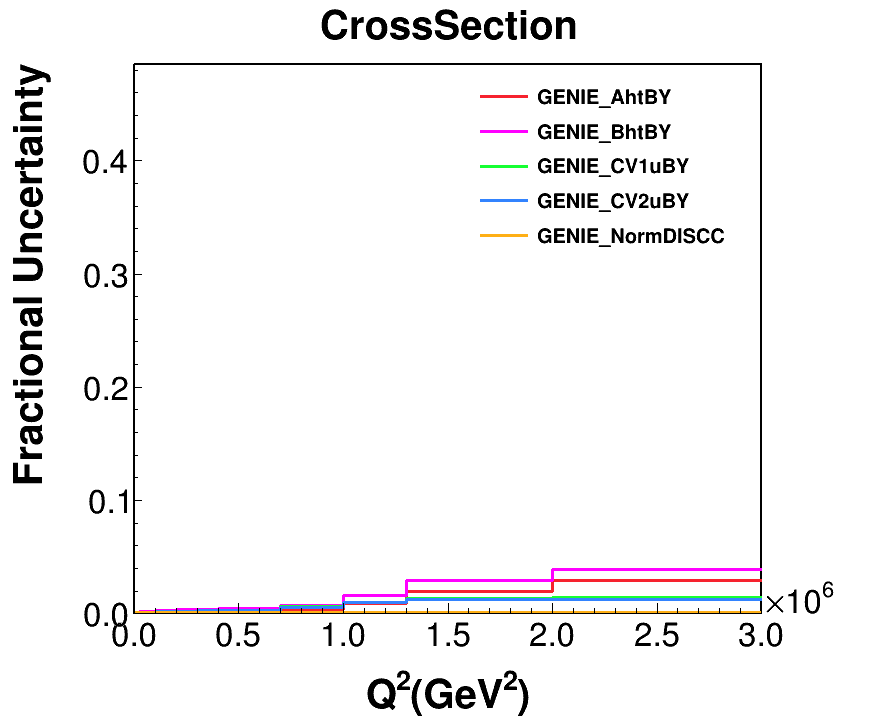
\includegraphics[scale=0.28]{Figures/AppendixB/XsecUnc1D/ErrorSummary_CrossSection_q2_Frac__1Pi_DIS-Hadronization.png}
        \caption{$\NewVar$ 1D cross section systematic error breakdown for the DIS and hadronization models.}
        \label{fig:AppendixB:CrossSecModel:1DCrossSectionDISHadronization\var}
    \end{figure}  
}


%\subsection{Elastic Cross Section Models Breakdown Uncertainties}
%\label{Ap:Systematics1D:CrosSectionModels:Elastic}

\foreach \var in  {enu,mixtpi,mixthetapi_deg,pmu,ptmu,pzmu,thetamu_deg,q2,wexp}{
%\foreach \var in  {enu_true,mixtpi_true,pmu_true,ptmu_true,pzmu_true,thetamu_deg_true,q2_true,wexp_true}{
    \ifthenelse{\equal{\var}{enu}}{
      \renewcommand{\NewVar}{E_\nu}
    }{}
    \ifthenelse{\equal{\var}{mixtpi}}{
      \renewcommand{\NewVar}{T_\pi}
    }{}
    \ifthenelse{\equal{\var}{mixthetapi_deg}}{
      \renewcommand{\NewVar}{\theta_\pi}
    }{}
    \ifthenelse{\equal{\var}{pmu}}{
      \renewcommand{\NewVar}{P_\mu}
    }{}
    \ifthenelse{\equal{\var}{ptmu}}{
      \renewcommand{\NewVar}{P^T_\mu}
    }{}
    \ifthenelse{\equal{\var}{pzmu}}{
      \renewcommand{\NewVar}{P^z_\mu}
    }{}
    \ifthenelse{\equal{\var}{thetamu_deg}}{
      \renewcommand{\NewVar}{\theta_\mu}
    }{}
    \ifthenelse{\equal{\var}{q2}}{
      \renewcommand{\NewVar}{Q^2}
    }{}
    \ifthenelse{\equal{\var}{wexp}}{
      \renewcommand{\NewVar}{W_{exp}}
    }{}
    \begin{figure}[!h]
        \centering
        \includegraphics[scale=0.28]{Figures/AppendixB/XsecUnc1D/ErrorSummary_CrossSection_\var_Frac__1Pi_Elastic.png}
        \caption{$\NewVar$ 1D cross section systematic error breakdown for the Elastic interaction models.}
        \label{fig:AppendixB:CrossSecModel:1DCrossSectionElastic\var}
    \end{figure}  
}
\clearpage

%\subsection{MnvTunes Cross Section Models Breakdown Uncertainties}
%\label{Ap:Systematics1D:CrosSectionModels:MnvTunes}

\foreach \var in  {enu,mixtpi,mixthetapi_deg,pmu,ptmu,pzmu,thetamu_deg,q2,wexp}{
%\foreach \var in  {enu_true,mixtpi_true,pmu_true,ptmu_true,pzmu_true,thetamu_deg_true,q2_true,wexp_true}{
    \ifthenelse{\equal{\var}{enu}}{
      \renewcommand{\NewVar}{E_\nu}
    }{}
    \ifthenelse{\equal{\var}{mixtpi}}{
      \renewcommand{\NewVar}{T_\pi}
    }{}
    \ifthenelse{\equal{\var}{mixthetapi_deg}}{
      \renewcommand{\NewVar}{\theta_\pi}
    }{}
    \ifthenelse{\equal{\var}{pmu}}{
      \renewcommand{\NewVar}{P_\mu}
    }{}
    \ifthenelse{\equal{\var}{ptmu}}{
      \renewcommand{\NewVar}{P^T_\mu}
    }{}
    \ifthenelse{\equal{\var}{pzmu}}{
      \renewcommand{\NewVar}{P^z_\mu}
    }{}
    \ifthenelse{\equal{\var}{thetamu_deg}}{
      \renewcommand{\NewVar}{\theta_\mu}
    }{}
    \ifthenelse{\equal{\var}{q2}}{
      \renewcommand{\NewVar}{Q^2}
    }{}
    \ifthenelse{\equal{\var}{wexp}}{
      \renewcommand{\NewVar}{W_{exp}}
    }{}
    \begin{figure}[!h]
        \centering
        \includegraphics[scale=0.28]{Figures/AppendixB/XsecUnc1D/ErrorSummary_CrossSection_\var_Frac__1Pi_MnvTunes.png}
        \caption{$\NewVar$ 1D cross section systematic error breakdown for the MnvTunes models.}
        \label{fig:AppendixB:CrossSecModel:1DCrossSectionMnvTunes\var}
    \end{figure}  
}
\clearpage



%\subsection{No Resonant pion production Cross Section Models Breakdown Uncertainties}
%\label{Ap:Systematics1D:CrosSectionModels:NoRESpi}

\foreach \var in  {enu,mixtpi,mixthetapi_deg,pmu,ptmu,pzmu,thetamu_deg,q2,wexp}{
%\foreach \var in  {enu_true,mixtpi_true,pmu_true,ptmu_true,pzmu_true,thetamu_deg_true,q2_true,wexp_true}{
    \ifthenelse{\equal{\var}{enu}}{
      \renewcommand{\NewVar}{E_\nu}
    }{}
    \ifthenelse{\equal{\var}{mixtpi}}{
      \renewcommand{\NewVar}{T_\pi}
    }{}
    \ifthenelse{\equal{\var}{mixthetapi_deg}}{
      \renewcommand{\NewVar}{\theta_\pi}
    }{}
    \ifthenelse{\equal{\var}{pmu}}{
      \renewcommand{\NewVar}{P_\mu}
    }{}
    \ifthenelse{\equal{\var}{ptmu}}{
      \renewcommand{\NewVar}{P^T_\mu}
    }{}
    \ifthenelse{\equal{\var}{pzmu}}{
      \renewcommand{\NewVar}{P^z_\mu}
    }{}
    \ifthenelse{\equal{\var}{thetamu_deg}}{
      \renewcommand{\NewVar}{\theta_\mu}
    }{}
    \ifthenelse{\equal{\var}{q2}}{
      \renewcommand{\NewVar}{Q^2}
    }{}
    \ifthenelse{\equal{\var}{wexp}}{
      \renewcommand{\NewVar}{W_{exp}}
    }{}
    \begin{figure}[!h]
        \centering
        \includegraphics[scale=0.28]{Figures/AppendixB/XsecUnc1D/ErrorSummary_CrossSection_\var_Frac__1Pi_NonRESPi.png}
        \caption{$\NewVar$ 1D cross section systematic error breakdown for the no resonant pion models.}
        \label{fig:AppendixB:CrossSecModel:1DCrossSectionNoRESpi\var}
    \end{figure}  
}




%\subsection{Resonant pion production Cross Section Models Breakdown Uncertainties}
%\label{Ap:Systematics1D:CrosSectionModels:RESpi}
\foreach \var in  {enu,mixtpi,mixthetapi_deg,pmu,ptmu,pzmu,thetamu_deg,q2,wexp}{
%\foreach \var in  {enu_true,mixtpi_true,pmu_true,ptmu_true,pzmu_true,thetamu_deg_true,q2_true,wexp_true}{
    \ifthenelse{\equal{\var}{enu}}{
      \renewcommand{\NewVar}{E_\nu}
    }{}
    \ifthenelse{\equal{\var}{mixtpi}}{
      \renewcommand{\NewVar}{T_\pi}
    }{}
    \ifthenelse{\equal{\var}{mixthetapi_deg}}{
      \renewcommand{\NewVar}{\theta_\pi}
    }{}
    \ifthenelse{\equal{\var}{pmu}}{
      \renewcommand{\NewVar}{P_\mu}
    }{}
    \ifthenelse{\equal{\var}{ptmu}}{
      \renewcommand{\NewVar}{P^T_\mu}
    }{}
    \ifthenelse{\equal{\var}{pzmu}}{
      \renewcommand{\NewVar}{P^z_\mu}
    }{}
    \ifthenelse{\equal{\var}{thetamu_deg}}{
      \renewcommand{\NewVar}{\theta_\mu}
    }{}
    \ifthenelse{\equal{\var}{q2}}{
      \renewcommand{\NewVar}{Q^2}
    }{}
    \ifthenelse{\equal{\var}{wexp}}{
      \renewcommand{\NewVar}{W_{exp}}
    }{}
    \begin{figure}[!h]
        \centering
        \includegraphics[scale=0.28]{Figures/AppendixB/XsecUnc1D/ErrorSummary_CrossSection_\var_Frac__1Pi_RESPi.png}
        \caption{$\NewVar$ 1D cross section systematic error breakdown for the Resonant pion production models.}
        \label{fig:AppendixB:CrossSecModel:1DCrossSectionRESpi\var}
    \end{figure}  
}

\pagebreak

\section{Genie FSI Uncertainties}
\label{Ap:Systematics1D:FSI}

\foreach \var in  {enu,mixtpi,mixthetapi_deg,pmu,ptmu,pzmu,thetamu_deg,q2,wexp}{
%\foreach \var in  {enu_true,mixtpi_true,pmu_true,ptmu_true,pzmu_true,thetamu_deg_true,q2_true,wexp_true}{
    \ifthenelse{\equal{\var}{enu}}{
      \renewcommand{\NewVar}{E_\nu}
    }{}
    \ifthenelse{\equal{\var}{mixtpi}}{
      \renewcommand{\NewVar}{T_\pi}
    }{}
    \ifthenelse{\equal{\var}{mixthetapi_deg}}{
      \renewcommand{\NewVar}{\theta_\pi}
    }{}
    \ifthenelse{\equal{\var}{pmu}}{
      \renewcommand{\NewVar}{P_\mu}
    }{}
    \ifthenelse{\equal{\var}{ptmu}}{
      \renewcommand{\NewVar}{P^T_\mu}
    }{}
    \ifthenelse{\equal{\var}{pzmu}}{
      \renewcommand{\NewVar}{P^z_\mu}
    }{}
    \ifthenelse{\equal{\var}{thetamu_deg}}{
      \renewcommand{\NewVar}{\theta_\mu}
    }{}
    \ifthenelse{\equal{\var}{q2}}{
      \renewcommand{\NewVar}{Q^2}
    }{}
    \ifthenelse{\equal{\var}{wexp}}{
      \renewcommand{\NewVar}{W_{exp}}
    }{}
    \begin{figure}[!h]
        \centering
        \includegraphics[scale=0.28]{Figures/AppendixB/XsecUnc1D/ErrorSummary_CrossSection_\var_Frac__1Pi_GENIE_FSI.png}
        \caption{$\NewVar$ 1D cross section systematic error breakdown for the FSI models.}
        \label{fig:AppendixB:CrossSecModel:1DFSImodel\var}
    \end{figure}  
}
\clearpage




%\subsection{CCQE Cross Section Models Breakdown Uncertainties}
%\label{Ap:Systematics1D:CrosSectionModels:CCQE}



\pagebreak


\section{Muon Uncertainties}
\label{Ap:Systematics1D:Muon}

\foreach \var in  {enu,mixtpi,mixthetapi_deg,pmu,ptmu,pzmu,thetamu_deg,q2,wexp}{
%\foreach \var in  {enu_true,mixtpi_true,pmu_true,ptmu_true,pzmu_true,thetamu_deg_true,q2_true,wexp_true}{
    \ifthenelse{\equal{\var}{enu}}{
      \renewcommand{\NewVar}{E_\nu}
    }{}
    \ifthenelse{\equal{\var}{mixtpi}}{
      \renewcommand{\NewVar}{T_\pi}
    }{}
    \ifthenelse{\equal{\var}{mixthetapi_deg}}{
      \renewcommand{\NewVar}{\theta_\pi}
    }{}
    \ifthenelse{\equal{\var}{pmu}}{
      \renewcommand{\NewVar}{P_\mu}
    }{}
    \ifthenelse{\equal{\var}{ptmu}}{
      \renewcommand{\NewVar}{P^T_\mu}
    }{}
    \ifthenelse{\equal{\var}{pzmu}}{
      \renewcommand{\NewVar}{P^z_\mu}
    }{}
    \ifthenelse{\equal{\var}{thetamu_deg}}{
      \renewcommand{\NewVar}{\theta_\mu}
    }{}
    \ifthenelse{\equal{\var}{q2}}{
      \renewcommand{\NewVar}{Q^2}
    }{}
    \ifthenelse{\equal{\var}{wexp}}{
      \renewcommand{\NewVar}{W_{exp}}
    }{}
    \begin{figure}[!h]
        \centering
        \includegraphics[scale=0.28]{Figures/AppendixB/XsecUnc1D/ErrorSummary_CrossSection_\var_Frac__1Pi_Muon.png}
        \caption{$\NewVar$ 1D cross section systematic error breakdown for the associated muon kinematics measurements. }
        \label{fig:AppendixB:CrossSecModel:1DMuon\var}
    \end{figure}  
}
\clearpage



\section{Pion Reconstruction Uncertainties}
\label{Ap:Systematics1D:PionReconstruction}

\foreach \var in  {enu,mixtpi,mixthetapi_deg,pmu,ptmu,pzmu,thetamu_deg,q2,wexp}{
%\foreach \var in  {enu_true,mixtpi_true,pmu_true,ptmu_true,pzmu_true,thetamu_deg_true,q2_true,wexp_true}{
    \ifthenelse{\equal{\var}{enu}}{
      \renewcommand{\NewVar}{E_\nu}
    }{}
    \ifthenelse{\equal{\var}{mixtpi}}{
      \renewcommand{\NewVar}{T_\pi}
    }{}
    \ifthenelse{\equal{\var}{mixthetapi_deg}}{
      \renewcommand{\NewVar}{\theta_\pi}
    }{}
    \ifthenelse{\equal{\var}{pmu}}{
      \renewcommand{\NewVar}{P_\mu}
    }{}
    \ifthenelse{\equal{\var}{ptmu}}{
      \renewcommand{\NewVar}{P^T_\mu}
    }{}
    \ifthenelse{\equal{\var}{pzmu}}{
      \renewcommand{\NewVar}{P^z_\mu}
    }{}
    \ifthenelse{\equal{\var}{thetamu_deg}}{
      \renewcommand{\NewVar}{\theta_\mu}
    }{}
    \ifthenelse{\equal{\var}{q2}}{
      \renewcommand{\NewVar}{Q^2}
    }{}
    \ifthenelse{\equal{\var}{wexp}}{
      \renewcommand{\NewVar}{W_{exp}}
    }{}
    \begin{figure}[!h]
        \centering
        \includegraphics[scale=0.28]{Figures/AppendixB/XsecUnc1D/ErrorSummary_CrossSection_\var_Frac__1Pi_Pion_Reconstruction.png}
        \caption{$\NewVar$ 1D cross section systematic error breakdown for the associated pion reconstruction. }
        \label{fig:AppendixB:CrossSecModel:1DPionReconstruction\var}
    \end{figure}  
}
\clearpage


\section{Flux Uncertainties}
\label{Ap:Systematics1D:Flux}

\foreach \var in  {enu,mixtpi,mixthetapi_deg,pmu,ptmu,pzmu,thetamu_deg,q2,wexp}{
%\foreach \var in  {enu_true,mixtpi_true,pmu_true,ptmu_true,pzmu_true,thetamu_deg_true,q2_true,wexp_true}{
    \ifthenelse{\equal{\var}{enu}}{
      \renewcommand{\NewVar}{E_\nu}
    }{}
    \ifthenelse{\equal{\var}{mixtpi}}{
      \renewcommand{\NewVar}{T_\pi}
    }{}
    \ifthenelse{\equal{\var}{mixthetapi_deg}}{
      \renewcommand{\NewVar}{\theta_\pi}
    }{}
    \ifthenelse{\equal{\var}{pmu}}{
      \renewcommand{\NewVar}{P_\mu}
    }{}
    \ifthenelse{\equal{\var}{ptmu}}{
      \renewcommand{\NewVar}{P^T_\mu}
    }{}
    \ifthenelse{\equal{\var}{pzmu}}{
      \renewcommand{\NewVar}{P^z_\mu}
    }{}
    \ifthenelse{\equal{\var}{thetamu_deg}}{
      \renewcommand{\NewVar}{\theta_\mu}
    }{}
    \ifthenelse{\equal{\var}{q2}}{
      \renewcommand{\NewVar}{Q^2}
    }{}
    \ifthenelse{\equal{\var}{wexp}}{
      \renewcommand{\NewVar}{W_{exp}}
    }{}
    \begin{figure}[!h]
        \centering
        \includegraphics[scale=0.28]{Figures/AppendixB/XsecUnc1D/ErrorSummary_CrossSection_\var_Frac__1Pi_Flux.png}
        \caption{$\NewVar$ 1D cross section systematic error breakdown for the associated to the neutrino flux.}
        \label{fig:AppendixB:CrossSecModel:1DFlux\var}
    \end{figure}  
}
\clearpage

\section{Others Uncertainties}
\label{Ap:Systematics1D:Others}

\foreach \var in  {enu,mixtpi,mixthetapi_deg,pmu,ptmu,pzmu,thetamu_deg,q2,wexp}{
%\foreach \var in  {enu_true,mixtpi_true,pmu_true,ptmu_true,pzmu_true,thetamu_deg_true,q2_true,wexp_true}{
    \ifthenelse{\equal{\var}{enu}}{
      \renewcommand{\NewVar}{E_\nu}
    }{}
    \ifthenelse{\equal{\var}{mixtpi}}{
      \renewcommand{\NewVar}{T_\pi}
    }{}
    \ifthenelse{\equal{\var}{mixthetapi_deg}}{
      \renewcommand{\NewVar}{\theta_\pi}
    }{}
    \ifthenelse{\equal{\var}{pmu}}{
      \renewcommand{\NewVar}{P_\mu}
    }{}
    \ifthenelse{\equal{\var}{ptmu}}{
      \renewcommand{\NewVar}{P^T_\mu}
    }{}
    \ifthenelse{\equal{\var}{pzmu}}{
      \renewcommand{\NewVar}{P^z_\mu}
    }{}
    \ifthenelse{\equal{\var}{thetamu_deg}}{
      \renewcommand{\NewVar}{\theta_\mu}
    }{}
    \ifthenelse{\equal{\var}{q2}}{
      \renewcommand{\NewVar}{Q^2}
    }{}
    \ifthenelse{\equal{\var}{wexp}}{
      \renewcommand{\NewVar}{W_{exp}}
    }{}
    \begin{figure}[!h]
        \centering
        \includegraphics[scale=0.28]{Figures/AppendixB/XsecUnc1D/ErrorSummary_CrossSection_\var_Frac__1Pi_Others.png}
        \caption{$\NewVar$ 1D cross section systematic error breakdown. }
        \label{fig:AppendixB:CrossSecModel:1DOther\var}
    \end{figure}  
}
\clearpage



 
%&&&&&&&&&&&&&&&&&&&&&&&&&&&&&&&&&&&&&&&&&&&&&&&&&&&&&&&&&&&&&&&&&&&&&&&&&&&&&&
%       Bibliografa.
%&&&&&&&&&&&&&&&&&&&&&&&&&&&&&&&&&&&&&&&&&&&&&&&&&&&&&&&&&&&&&&&&&&&&&&&&&&&&&&
    
	\bibliographystyle{unsrtnat}
	\bibliography{./Biblio/References}
	\addcontentsline{toc}{chapter}{Bibliografía.}

\end{document}
%==============================================================================
%==============================================================================